            % ****** Start of file apssamp.tex ******
%
%   This file is part of the APS files in the REVTeX 4.2 distribution.
%   Version 4.2a of REVTeX, December 2014
%
%   Copyright (c) 2014 The American Physical Society.
%
%   See the REVTeX 4 README file for restrictions and more information.
%
% TeX'ing this file requires that you have AMS-LaTeX 2.0 installed
% as well as the rest of the prerequisites for REVTeX 4.2
%
% See the REVTeX 4 README file
% It also requires running BibTeX. The commands are as follows:
%
%  1)  latex apssamp.tex
%  2)  bibtex apssamp
%  3)  latex apssamp.tex
%  4)  latex apssamp.tex
%
\documentclass[twocolumn,superscriptaddress,unsortedaddress,
%runinaddress,
%frontmatterverbose, 
%preprint,
%preprintnumbers,
%nofootinbib,
%nobibnotes,
%bibnotes,
 amsmath,amssymb,
 aps,
%pra,
%prb,
%rmp,
%prstab,
%prstper,
%floatfix,
]{revtex4-2}

\usepackage{graphicx,tikz} % Include figure files
\usepackage[mode=buildnew]{standalone} % For inclusion of .tex figures.
\usepackage{dcolumn}% Align table columns on decimal point
\usepackage{bm}% bold math
\usepackage{physics}
\usepackage{xcolor}
\usepackage{siunitx}
% \usepackage{braket}
\usetikzlibrary{external}
\usepackage{soul}
% \tikzexternalize[prefix=tikz/]

%\newcommand\abs[1]{\left|#1\right|}
%\newcommand\bra[1]{\left| #1 \right \rangle}
%\newcommand\ket[1]{\left \langle #1 \right |}

\newcommand{\may}[1]{\textcolor{orange}{#1}}
    % for marking stuff to be edited or verified later

\DeclareMathOperator{\sinc}{sinc}

\begin{document}

\preprint{APS/123-QED}

\title{Coulomb interaction-driven entanglement of electrons on helium}

\author{Niyaz Beysengulov and Johannes Pollanen}
\email{beysengu@msu.edu}
\email{pollanen@msu.edu}
\affiliation{Department of Physics and Astronomy, Michigan State University, East Lansing, MI 48824, USA}
\author{Øyvind Sigmundson Schøyen, Stian Dysthe Bilek, Jonas Boym Flaten, and Oskar Leinonen}
\affiliation{Department of Physics and Center for Computing in Science Education, University of Oslo, N-0316 Oslo, Norway}
\author{Håkon Emil Kristiansen}
\affiliation{Department of Chemistry and Hylleraas Center for Quantum Molecular Sciences, University of Oslo, N-0316 Oslo, Norway}
\author{Zachary Stewart, Jared Weidman, and Angela Wilson}
\affiliation{Department of Chemistry, Michigan State University, East Lansing, MI 48824, USA}
\author{Morten Hjorth-Jensen}
\affiliation{Facility for Rare Isotope Beams and Department of Physics and Astronomy, Michigan State University, East Lansing, MI 48824, USA}
\affiliation{Department of Physics and Center for Computing in Science Education, University of Oslo, N-0316 Oslo, Norway}
\begin{abstract}
  Here we describe a method for generating motional entanglement between two electrons trapped above the surface of superfluid helium. In this proposed scheme these electronic charge qubits are laterally confined via electrostatic gates to create an anharmonic trapping potential. When the system is cooled to sufficiently low temperature these in-plane charge qubit states are quantized and circuit quantum electrodynamic methods can be used to control and readout single qubit operations. Entangle gates are generated via the long-range Coulomb interaction between the two electrons and are modeled via a ...
\end{abstract}

\pacs{02.70.Ss, 31.15.A-, 31.15.bw, 71.15.-m, 73.21.La}


\date{\today}% It is always \today, today,
             %  but any date may be explicitly specified


                              %display desired
\maketitle

%\tableofcontents
\section{Introduction} % Morten + Johannes + Niyaz
Entanglement is the fundamental characteristic that distinguishes
quantum systems composed of two or more coupled objects from their classical counterparts. The study of entanglement in precisely engineered quantum systems with countably many degrees of freedom is at the forefront of modern physics and is a key resource in quantum information science (QIS). This is particularly true in the development of two-qubit logic for quantum computation. In fact, the generation of two-qubit entanglement has been demonstrated in a wide variety of physical systems used in present-day quantum computing, including superconducting circuits~\cite{Steffen1423,Barends2014}, trapped ions~\cite{Monroe1995,Schmidt-Kaler2003}, semiconductor quantum dots~\cite{Li809,Petta2005}, color-center defects in diamond~\cite{Dutt2007,Neumann2010,Bernien2013}, and neutral atoms in optical lattices~\cite{Levine2019,Madjarov2020} just to name a few. Investigating the generation and evolution of entanglement in quantum many-body systems is also important for quantum simulation~\cite{feynman1982simulating,Trabesinger2012,Georgescu2014,Altman2021}, having the potential to advance the fundamental understanding of dense nuclear matter or high-energy physics~\cite{Carlson2018,Klco2020,Yamamoto2022,Illa2022,Bauer2022}, correlated electron systems~\cite{Smith2016,Hofstetter2018,Smith2019}, and quantum chemistry~\cite{Peruzzo2014,Reiher2016,Kandala2017}. Quantum simulators based on ``natural'' qubits such as atoms~\cite{Greiner2002,Hart2015,Ebadi2021}, ions~\cite{Lanyon2011,Monroe2021} and photons~\cite{Aspuru-Guzik2012} are particularly appealing since these systems are highly programmable, controllable and replicable~\cite{Alsing2023}. Additionally, in these systems the coupling to decohering environmental degrees of freedom is minimal allowing for a tight feedback between simulator experiments and theory.

Trapped electron systems represent a novel approach to investigating the generation of entanglement and  quantum simulation sharing many of the features platforms based on other ``natural'' qubit. Recent experimental efforts have investigated the feasibility of trapped electron qubits using ion trap techniques~\cite{Matthiesen2019,Yu2022}. In contrast, the quantized motion of electrons naturally trapped in vacuum above the surface of superfluid helium was one of the earliest theoretical proposal for building a large scale analog quantum computer~\cite{platzman1999quantum}. The surface of the superfluid functions as a pristine substrate~\cite{Shirahama1995}, shielding the electrons from deleterious source of noise at the device layer beneath the helium. Since this initial work a number of theoretical proposal have been put forward to create both charge~\cite{dykman2003qubits,Dahm2003,Schuster2010,Shi2014,Kawakami2023} and spin~\cite{Lyon2006,Schuster2010,Dykman2023,Kawakami2023} qubits based on these trapped electrons. Additionally a wide variety of experimental work, directed at realizing these electronic qubits, has been performed to leverage advances in nano-fabrication techniques for precision trapping and control of electrons on helium in confined geometries~\cite{Marty1986,Ikegami2009,Rees2016a,Rees2016b,Zou2022}, mesoscopic devices~\cite{Papageorgiou2004,Rees2011,Rees2012}, circuit quantum electrodynamic architectures~\cite{Yang2016,koolstra2019coupling}, and surface acoustic wave devices~\cite{Byeon2021}. Single-electron trapping and detection has been experimentally achieved~\cite{Papageorgiou2004,Rousseau2007,koolstra2019coupling} as well as extremely high-fidelity, electron transfer along gated arrays fabricated using standard CMOS processes~\cite{Bradbury2011}. Similarly, electrons trapped above the surface of solidified noble gases offer an alternative trapped electron qubit. In fact, electrons trapped in vacuum above the surface of solid neon have recently been experimentally demonstrated as a novel ``natural'' charge qubit~\cite{} with high coherence~\cite{}. 

In aggregate these technological advances have opened the door to exploring the generation of entanglement in systems based on trapped electrons and the creation of a novel quantum simulator. This is particularly true for the system of electrons trapped above the surface of helium since the electron on the superfluid substrate are mobile,  precisely reconfigurable~\cite{}. Linear electron chains on helium are also home to highly connecting collective oscillations similar to those observed in ion trap systems, but with frequencies three orders of magnitude larger due to much lighter electron mass. Additionally, the electrons in this system are quantum non-degenerate and highly unscreened, making electrons on helium a paradigm for studying the generation of entanglement produced purely by the Coulomb interaction.



\may{{Here we show ... Could someone add 3-4 bulleted points here}}
\begin{itemize}
    \item How an effective double-well potential can be constructed from seven
        anodes underneath a liquid helium surface.
        % TODO: Someone with more understanding than me regarding this process
        % should improve on this point.
    \item How we can construct a two-qubit architecture by trapping a single
        electron in each well, with always-on Coulomb interaction.
    \item How the anodes can be tuned to make the system two effective single
        qubits, and perform a two-qubit gate.
\end{itemize}








Generating entanglement between two quantum systems rely on exploiting interactions in a controllable way. The details in the interaction Hamiltonian between two systems defines the protocol schemes for two-qubit logic. In superconducting circuits the interaction between qubits may arise from direct capacitive coupling between circuit elements or by indirect coupling of two qubits to a common resonator (virtually populating resonator mode) which results in a non-local Hamiltonian in the form of exchange interaction~\cite{blais2020circuit}. This allows us to implement various schemes for entanglement, such as $\sqrt{i\text{SWAP}}$ gate~\cite{bialczak2010quantum}, controlled-phase gate~\cite{dicarlo2009demonstration}, resonator-induced phase gate~\cite{paik2016experimental}, cross-resonance gate~\cite{chow2011simple} etc. Entanglement gates in trapped ions are produced by means of the Coulomb interaction, where shared motional modes of two or more ions, entangled to their internal states, used for transferring excitations between ion qubits~\cite{cirac1995quantum}. This has been experimentally demonstrated by implementing Cirac-Zoller gate~\cite{turchette1998deterministic}, Leibfried’s geometric-phase gate~\cite{leibfried2003experimental} etc. In photonic quantum computing schemes two-qubit entangling operations are realized by nonlinear interactions between two photons scattering from quantum dots, plasmonic nanowires, diamond vacancy centers and others embedded into waveguides~\cite{bartlett2020universal}. Two-qubit gates in semiconductor quantum dots are based on spin-spin exchange interactions~\cite{brunner2011two,watson2018programmable} or generated by coupling to a superconducting resonator via artificial spin-orbit interaction~\cite{borjans2020resonant}.

In the system of charge qubits one can generate entanglement via Coulomb interaction, where state-dependent charge configuration in one qubit impose different electric fields on the other qubit. \textit{discuss several examples, working on it, Niyaz}

Coulomb interaction governed entanglement naturally can be realized in the system of electrons on the surface of superfluid helium, where qubit states are formed by in-plane lateral motional or out-of plane Rydberg states. Trapped near the surface of liquid helium these states have different spatial charge configurations and the wavefunctions of different electrons do not overlap. This results in a strong exchange free Coulomb interaction which depends on the states of the electrons~\cite{dykman2003qubits}. The lack of disorder in the systems also leads to slow electron decoherence, which has attracted interest to the system as a candidate for quantum information processing~\cite{platzman1999quantum,lyon2006spin,schuster2010proposal}. Advances in micro- and nano-fabrication techniques have opened the door for the study of electrons on helium in confined geometries and mesoscopic devices. Single-electron detection has been experimentally achieved~\cite{glasson2005trapping,koolstra2019coupling} along with stable, high-fidelity, electron transfer along a gated CCD array~\cite{bradbury2011efficient}. Filamentation of electron current was observed in helium-filled microchannels along with electron crystallization and ``slip-stick'' dynamics of the Wigner solid~\cite{glasson2001observation,rees2016structural,rees2016stick}, where strong Coulomb interactions driven many-body phenomena were explored.


Electrons on helium is another qubit platform. Here 2 qubit gates have never been discussed in a proper manner.

The static Coulomb interaction arises from a virtual photon exchange process between two charge particles according to quantum electrodynamics. This results in a correlated motion of two charges generating quantum entanglement.
 / Forster interaction

Understanding the behavior of strongly confined electrons is of fundamental
interest for solving many-body problems.  Quantum dots, e.g. electrons
confined in semiconducting heterostructures, are of particular interest since
they exhibit, due to their small size, discrete quantum levels.  Under these
conditions, typical quantum phenomena like tunneling, entanglement and
magnetization can all be observed.   Since quantum
dots are manufactured and designed artificially at the laboratory, their
quantum levels can be arbitrarily tuned by changing the external field or the
size and shape of the system.  As a consequence, quantum dots provide a high
level of control for the dynamics and correlation of the electrons, which
makes them perfectly suited to study quantum effects in practice.  Since their
ground state shows similar shell structures and magic numbers as seen for
atoms and nuclei, these systems give the opportunity to
study electronic systems without the presence of a nucleus affecting the
electrons.  Apart from their relevance for theoretical research in quantum
physics, quantum dots offer a wide variety of applications: In particular,
their electrical and optical properties make them attractive for the use in
laser technology \cite{strauf2010,5075760} and solar cells
\cite{jenks:013111,doi:10.1021/cr900289f}, but they are also used in quantum
computers\cite{PhysRevA.57.120} and medical imaging \cite{Ben-Ari02042003}.


Our work's place in this field

%Electrons on helium represent a promising platform for investigating strongly-coupled qubits. Therefore a systematic investigation of the controlled generation of entanglement between two trapped electrons under the influence of coherent microwave driving pulses, taking into account the effects of the Coulomb interaction between electrons, is of significant importance for quantum information processing using trapped electrons.

\section{Device prototype}\label{sec:device} % Niyaz writes this
%general information about electrons on helium
Surface state electrons (SSE) 'floating' above liquid helium originates from quantization of electron's perpendicular to the surface motion in a trapping potential formed by attractive force from image charge and a large $\sim$1~eV barrier at the liquid-vacuum interface \cite{cole1969,shikin1971}. At low temperatures the SSE are trapped in the lowest Rydberg state for vertical motion some 11~nm above the helium surface, which is perfectly clean and has a permittivity close to that of vacuum. The weak interaction with enviorment, which is mainly governed by interactions with thermally excited capillary waves on the helium surface (ripplons) and bulk phonons, ensures long coherence times of a spin and motional degrees of freedom of electronic states \cite{dykman2003qubits,lyon2006spin}. SSE's in-plane motion can be further localized by using microdevices on the length scales approaching the interelectron separation (at the order of one micron) \cite{rees2011point,rees2016structural} and single electron trapping have been experimentally demonstrated \cite{Papageorgiou2005Counting,koolstra2019coupling,zhou2022single}. In these devices an unscreened Coulomb interactions between electrons give rise to a strongly correlated a two-dimensional electronic phase known as Wigner Solid \cite{rees2016structural,grimes1979evidence}. This strong interaction can be utilized as a source of entanglement and hybridize motional states of SSE's analogous to a Cirac-Zoller entangling gate.

The prototype system for measurements of two electron's in-plane motional state entanglement is sketched in Fig.~\ref{fig1}a. Here we consider a $3 \times 1$~$\mu$m$\times\mu$m size structure with a recess depth 0.5~$\mu$m, which is filled with superfluid helium via capillary action~\cite{marty1986stability}. Once the device is filled with helium, a thermionic emission from a tungsten filament located above the helium surface can be used to generate electrons, which will be naturally trapped at the liquid surface under positive bias voltage on the electrodes g1-7. We note, that trapping single or two electrons requires a controlled loading and unloading of electrons into the trap region from a larger area, where electrons are usually stored. This type of electron manipulations have been experimentally demonstrated in works refs. For the purpose of the current study we consider a simple gate array which allow a demonstration of entanglement between two electrons. The chip design and distances are chosen to promote a quantization axis along $x$ direction and keeping electron motional states along $y$-axis at sufficiently higher energies. Seven 200~nm-wide electrodes with 200~nm gap beneath the helium layer gives enough degrees of freedom to form a double-well electrostatic confinement. The electrostatic potential at the trap region is defined as
        \begin{align}
            \varphi(x, y) = \sum_{i=1}^7 \alpha_i(x, y) V_i,
            \label{eq:trap}
        \end{align}
where $\alpha_i = C_i/C_{\sum}$ is the relative contribution defined by a capacitances of the region of space at $(x, y)$ on the helium surface to the corresponding electrodes shown in Fig~\ref{fig1}b and $C_{\sum} = \sum_i C_i$. $V_i$ are voltages applied to gate electrodes with top electrodes kept at the ground potential. The coupling constants $\alpha_i (x, y)$ are calculated by numerically solving Laplace equation for electrostatic potential using Finite Element Modelling techniques. In our scheme the double-well is achieved by providing a negative potential to the central electrode (electrode 4 in Fig.~\ref{fig1}a) with a more positive potentials applied to other electrodes. The particular choice of the applied voltage will be described in a Section IV.


\textit{Niyaz / Introduce hamiltonian}

\begin{figure}
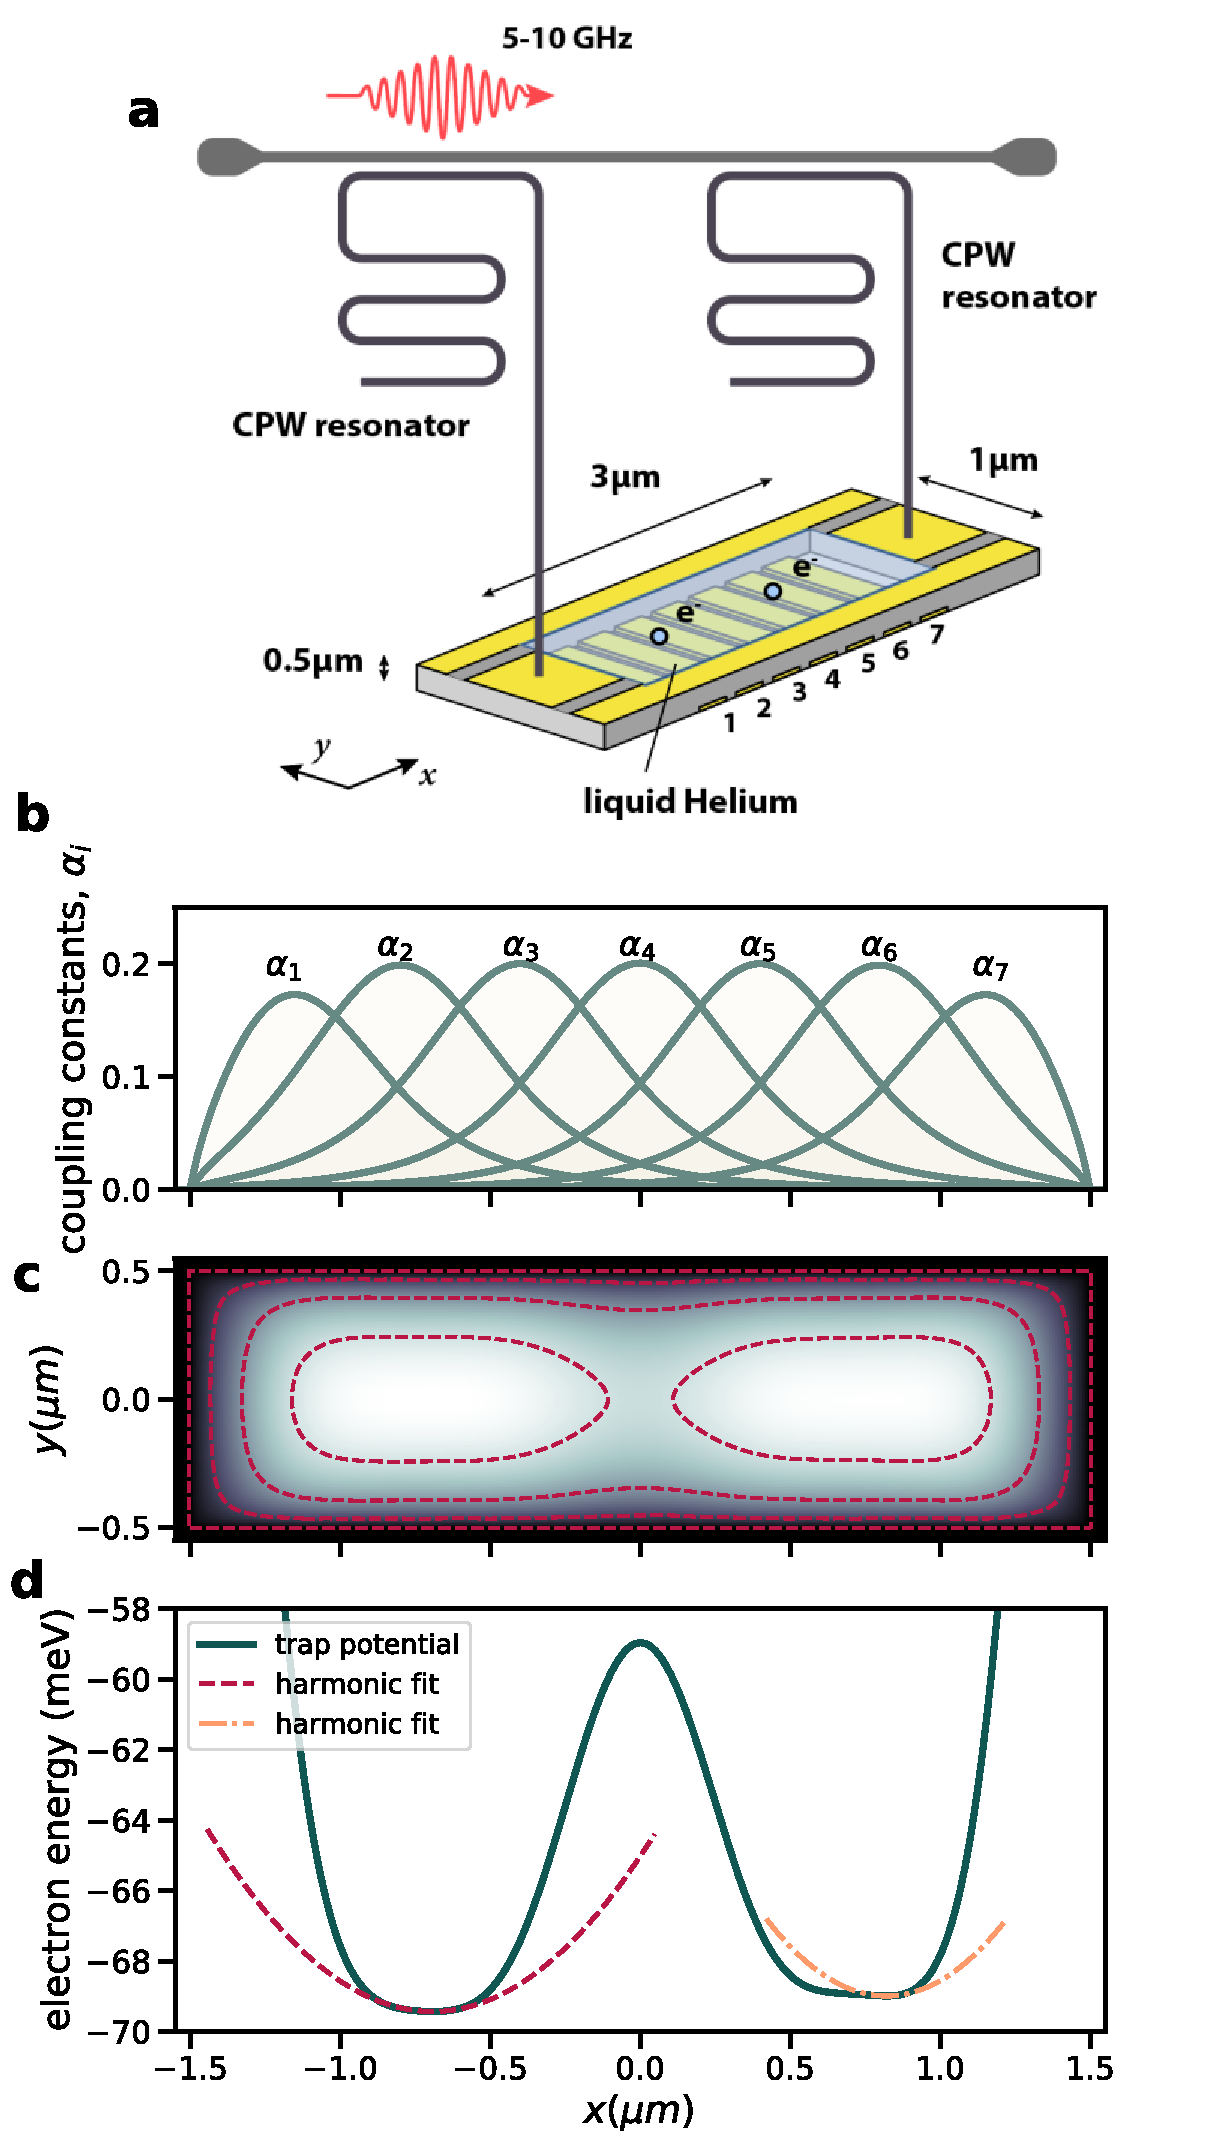
\includegraphics[width=\columnwidth]{figures/figure1.pdf}
\caption{\label{fig1} (a) Schematic of the microdevice, where two electrons are trapped in a double-well potential created by electrodes 1-7. The read-out is provided by two superconducting resonators dispersively coupled to  electron's in-plane motional states. (b) Coupling constants from each individual electrode beneath the helium layer. (c) The electron's energy in a  double-well electrostatic potential (solid line). Dashed and dot-dashed lines represent the harmonic approximations of left and right wells respectively.}
\end{figure}

The electron motional states read-out scheme is shown on Fig.~\ref{fig1}a and is based on the coupling of motional states to the photons in the superconducting resonator. We estimate the coupling energy to be $g/2 \pi = \langle 1 | d E| 0 \rangle \simeq $. The largest contribution to the decoherence is realized via energy decay into phonons of the liquid helium, which was estimated to be. This allow the realization of the strong coupling regime $g \rangle \Gamma$. Each of the individual electrons coupled to its own cpw $\lambda/4$-resonator with different resonance frequencies. We estimate the crosstalk coupling of the electron to the other resonator to be, so we will ignore this. However this crosstalk will limit the fidelities of the gate and well developed the pulse shaping techniques can be used to mitigate this coupling. In a dispersive regime, realized at the condition, the frequency of the reonators becomes electron state-dependent, which can be measured via transmitted microwave signals through the cpw feedline.

% TODO: Add to appendix/supplemental material
% \section{Interaction driven entanglement}
% 
% In order to study the importance of level avoided crossings and
% entanglement, we study first a simple two-level system. Thereafter we
% extend our level-crossing model to a four-level system which can be
% interpreted as composed of two separate (not necessarily identical)
% subsystems.
% 
% We let our Hamiltonian depend linearly on a strength parameter $\lambda$
% \[
%        H=H_0+\lambda H_\mathrm{I},
% \]
% with $\lambda \in [0,1]$, where the limits $\lambda=0$ and $\lambda=1$
% represent the non-interacting (or unperturbed) and fully interacting
% system, respectively.  The model is an eigenvalue problem with only
% two available states, which we label $\vert 0\rangle$ and $\vert
% 1\rangle$, respectively. Below we will let state $\vert 0 \rangle$
% represent the lowest state (often referred to as model-space state)
% eigenvalue whereas state $\vert 1\rangle$ represents the eigenvalue of
% the excluded space.  The non-interacting solutions to our problem are
% 
% \[
%        H_0\vert 0 \rangle =\epsilon_0\vert 0 \rangle,
% \]
% and
% \[
%        H_0\vert 1\rangle =\epsilon_1\vert 1\rangle,
% \]
% with $\epsilon_0 < \epsilon_1$. We label the off-diagonal matrix
% elements $X$, while $X_0=\langle 0 \vert H_\mathrm{I}\vert 0 \rangle$ and
% $X_1=\langle 1 \vert H_\mathrm{I}\vert 1 \rangle$.  The Hamiltonian matrix to be diagonalized is then given by
% \[
% \left(\begin{array}{cc}\epsilon_0+\lambda X_0 &\lambda X \\
% \lambda X &\epsilon_1+\lambda X_1 \end{array}\right).
% \]
% 
% In the results below we set the parameters $\epsilon_0=0$,
% $\epsilon_1=4$, $X_0=-X_1=3$ and $X=0.2$.  This eigenvalue problem can
% easily be rewritten in terms of the standard Pauli matrices.  The
% non-interacting solutions represent our computational basis.
% Pertinent to our choice of parameters, is that at $\lambda\geq 2/3$,
% the lowest eigenstate is dominated by $\vert 1\rangle$ while the upper
% is $\vert 0 \rangle$. At $\lambda=1$ the $\vert 0 \rangle$ mixing of
% the lowest eigenvalue is $1\%$ while for $\lambda\leq 2/3$ we have a
% $\vert 0 \rangle$ component of more than $90\%$.  The character of the
% eigenvectors has therefore been interchanged when passing $z=2/3$. The
% value of the parameter $X$ represents the strength of the coupling
% between the model space and the excluded space.  
% % add figure here
% 
% This  model exhibits a simple level crossing where the
% composition of the final interacting states change character as we
% gradually switch on the interaction.  In order to study how
% entanglement relates to level crossing and the main results of our
% investigations, we extend the simple two-level system to a four level
% system. This system can be thought of as composed of two subsystems
% $A$ and $B$. Each subsystem has computational basis states
% 
% \[
% \vert 0\rangle_{\mathrm{A,B}}=\begin{bmatrix} 1 & 0\end{bmatrix}^T \hspace{1cm} \vert 1\rangle_{\mathrm{A,B}}=\begin{bmatrix} 0 & 1\end{bmatrix}^T.
% \]
% 
% The subsystems could represent single particles or composite many-particle systems of a given symmetry.
% This leads to the many-body computational basis states
% \[
% \vert 00\rangle = \vert 0\rangle_{\mathrm{A}}\otimes \vert 0\rangle_{\mathrm{B}}=\begin{bmatrix} 1 & 0 & 0 &0\end{bmatrix}^T,
% \]
% and
% \[
% \vert 10\rangle = \vert 1\rangle_{\mathrm{A}}\otimes \vert 0\rangle_{\mathrm{B}}=\begin{bmatrix} 0 & 1 & 0 &0\end{bmatrix}^T,
% \]
% and
% \[
% \vert 01\rangle = \vert 0\rangle_{\mathrm{A}}\otimes \vert 1\rangle_{\mathrm{B}}=\begin{bmatrix} 0 & 0 & 1 &0\end{bmatrix}^T,
% \]
% and finally
% \[
% \vert 11\rangle = \vert 1\rangle_{\mathrm{A}}\otimes \vert 1\rangle_{\mathrm{B}}=\begin{bmatrix} 0 & 0 & 0 &1\end{bmatrix}^T.
% \]
% These computational basis states define also the eigenstates of the non-interacting  Hamiltonian
% \[
% H_0\vert 00 \rangle = \epsilon_{00}\vert 00 \rangle,
% \]
% \[
% H_0\vert 10 \rangle = \epsilon_{10}\vert 10 \rangle,
% \]
% \[
% H_0\vert 01 \rangle = \epsilon_{01}\vert 01 \rangle,
% \]
% and
% \[
% H_0\vert 11 \rangle = \epsilon_{11}\vert 11 \rangle.
% \]
% The interacting part of the Hamiltonian $H_{\mathrm{I}}$ is given by the tensor product of two $\sigma_x$ and $\sigma_z$  matrices, respectively, that is
% \[
% H_{\mathrm{I}}=H_x\sigma_x\otimes\sigma_x+H_z\sigma_z\otimes\sigma_z,
% \]
% 
% where $H_x$ and $H_z$ are interaction strength parameters. Our final Hamiltonian matrix is given by
% \[
% \bm{H}=\begin{bmatrix} \epsilon_{00}+H_z & 0 & 0 & H_x \\
%                        0  & \epsilon_{10}-H_z & H_x & 0 \\
%                        0 & H_x & \epsilon_{01}+H_z & 0 \\
%                        H_x & 0 & 0 & \epsilon_{11} -H_z \end{bmatrix}.
% \]
% 
% The four eigenstates of the above Hamiltonian matrix can in turn be used to
% define density matrices. As an example, the density matrix of the
% first eigenstate (lowest energy $E_0$) $\Psi_0$ is
% 
% \[
% \rho_0=\left(\alpha_{00}\vert 00 \rangle\langle 00\vert+\alpha_{10}\vert 10 \rangle\langle 10\vert+\alpha_{01}\vert 01 \rangle\langle 01\vert+\alpha_{11}\vert 11\
%  \rangle\langle 11\vert\right),
% \]
% where the coefficients $\alpha_{ij}$ are the eigenvector coefficients
% resulting from the solution of the above eigenvalue problem.  We can
% then in turn define the density matrix for the subsets $A$ or $B$ as
% 
% \[
% \rho_A=\mathrm{Tr}_B(\rho_{0})=\langle 0 \vert \rho_{0} \vert 0\rangle_{B}+\langle 1 \vert \rho_{0} \vert 1\rangle_{B},
% \]
% or
% \[
% \rho_B=\mathrm{Tr}_A(\rho_{\Psi_0})=\langle 0 \vert \rho_{0} \vert 0\rangle_{A}+\langle 1 \vert \rho_{0} \vert 1\rangle_{A}.
% \]
% 
% The density matrices for these subsets can be used to compute the
% so-called von Neumann entropy, which is one of the possible measures
% of entanglement. A pure state has entropy equal zero while entangled
% state have an entropy larger than zero. The von Neumann entropy is
% defined as
% \[
% S(A,B)=-\mathrm{Tr}\left(\rho_{A,B}\log_2 (\rho_{A,B})\right).
% \]
% The example here shows the above von Neumann entropy based on the
% density matrix for the lowest many-body state. We see clearly a jump
% in the entropy around the point where we have a level crossing. At
% interaction strength $\lambda=0$ we have many-body states purely
% defined by their computational basis states. As we switch on the
% interaction strength, we obtain an increased degree of mixing and the
% entropy increases till we reach the level crossing point where we see
% an additional and sudden increase in entropy. Similar behaviors are
% observed for the other states. The most important result from this
% example is that entanglement is driven by the Hamiltonian itself and
% the strength of the interaction matrix elements and the
% non-interacting energies.
% 
% % add figs here
% 
% With these introductory examples, we are now in the position where we
% can start to interpret and model realistic interacting many-electron
% systems in terms of the strength of the Coulomb interaction and the
% shapes of the potential well. Our specific system is composed of two
% potential wells with one fermion (electrons in our case) trapped in
% each well.  Each potential well can sustain a certain number of bound
% single-particle states and defines our subsystems $A$ and $B$. The
% non-interacting part of the Hamiltonian is given by the mere addition
% of the single-particle energies from each respective well (make figure
% with labels A and B and single-particle energies).
% 
% The eigenstates of the non-interacting Hamiltonian $H_0$ are given by
% various computational basis states with the difference from the above
% simple models that now we have more than two states in each
% subsystem. The depths of the potential wells and their respective
% distances can be tuned in an experimental set up. The theoretical
% calculations presented here can thus serve as a tool which aids in
% finding the optimal parameters in order to study entanglement in a
% many-body environment.
% 
% What follows is a description of the theoretical models used to
% simulate the two-electron system. 

\section{Entanglement in quantum dot systems}
    To investigate our model, which consists of two electrons confined to a one-dimensional external potential, we utilized the method of exact diagonalization to solve the two-body Schrödinger equation.
    We build a two-particle wave function from a set of single-particle functions.
    The representation of the one-body Hamiltonian's eigenstates on a discrete grid offers us the flexibility to select the external potential of our choice, and it also fits the interpolated potential very effectively.
    % TODO: We need to describe the interpolation of the potential.

    \subsection{The Hamiltonian}
        The full Hamiltonian for two interacting electrons in an external
        potential $v(x)$ is given by
        \begin{align}
            \hat{H}/E_{\mathrm{d}}
            = \sum_{i = 1}^{2}\qty(
                -\frac{1}{2}\dv[2]{}{x_i}
                + v(x_i)
            )
            + u(x_1, x_2),
            \label{eq:hamiltonian}
        \end{align}
        where the dimensionless coordinates of the electrons are $x_i = x_i^{\mathrm{real}}/x_0$ with $x_0 = \SI{123}{\nm}$ being the characteristic length scale, and $E_{\mathrm{d}} = \hbar^2/m_{\mathrm{e}} x_0^2$ is the energy scale with $m_{\mathrm{e}}$ the electron mass.
        The external potential is given by $v(x) = -e \varphi(x) / E_{\mathrm{d}}$.
        We use a soft Coulomb-like interaction $u(x_1, x_2)$ given by
        \begin{align}
            u(x_1, x_2)
            =
            \frac{\kappa}{\sqrt{\qty(x_1 - x_2)^2 + a^2}}.
            \label{eq:soft-coulomb}
        \end{align}
        % TODO: Discuss dimensionality of the problem.
        % Note: Scaling should maybe be discussed in full when introducing kappa
        Here $\kappa = e^2/4 \pi \epsilon_0 E_{\mathrm{d}} = 2326$ defines the strength of the interaction, and a shielding parameter parameter $a=10^{-2}$ removes the singularity at $x_1 = x_2$.
        We note that the natural spin-orbit interaction is small due to relatively small effective magnetic field $B_{||} = -\mathbf{v}^{\mathrm{th}} \times \mathbf{E}_{\perp}/c^2 \approx \SI{1e-8}{\tesla}$ \cite{lyon2006spin}, where $\mathbf{v}^{\mathrm{th}} \approx \SI{600}{\meter\per\s}$ is a thermal velocity of the electron at $T = \SI{10}{\milli\kelvin}$ and $\mathbf{E}_{\perp} \approx \SI{1e6}{\volt\per\meter}$ is a typical pressing electric field the electron experiences in the potential well.
        Potentially the spin-orbit interaction can be artificially enhanced in the presence of the spatially inhomogeneous magnetic field applied along the helium surface and parallel to the dipole moment of the orbital state \cite{schuster2010proposal}, which will be addressed elsewhere. 
        We therefore restrict our attention to the spatial part of the Hamiltonian.

        The choice of $v(x)$ with sufficiently deep wells enforces no
        tunneling over the barrier for the bound states we are interested in. We write $v(x) = v^L(x) + v^R(x)$, with $L$ and $R$ denoting the left and the right well respectively.
        % TODO: Add figure of each well separatelely here?
        % Alternatively, add the sum of the two wells overlaid on the full double
        % well potential.
        Here we choose the individual potentials to be $v^L(x) = v^L(x_b)$
        for $x \geq x_b$, and $v^R(x) = v^R(x_b)$ for $x \leq x_b$ with $x_b$ being the location of the maximal value of the barrier.
        % TODO: Check this formula when v(x_b) != 0.
        % It is okay as long as the barrier goes to zero at its maximum point.
        This ensures each of $v^L(x)$ and $v^R(x)$ describes a single well, and as a result, the left well remains constant across the right well, and vice versa.
        Furthermore, as a result of the strong Coulomb interaction, there will be a significant energy gap between the states in which one electron is present in each well and the states in which both electrons occupy a single well.
        % TODO: Can we estimate how large this gap is?
        
        By entirely factoring out the spin component of the problem (as the singlet and triplet states will be degenerate), we can treat the two electrons as distinguishable particles, with one electron located in the left well and the other electron situated in the right well.
        The one-body Hamiltonian for each electron can then be written
        \begin{align}
            \hat{h}^A
            = -\frac{1}{2} \dv[2]{}{x}
            + v^A(x),
            \label{eq:one-body-hamiltonian}
        \end{align}
        with $A \in \qty{L, R}$, and the two-body Hamiltonian from
        Eq.~\eqref{eq:soft-coulomb}.

    \subsection{Constructing the single-particle basis sets}
        \label{sec:basis-set}
        \textcolor{red}{Q1} In order to accommodate a variable number of grid points, we adopt linear interpolation for the coupling constants. 
        % TODO: Perhaps placed better elsewhere
        \textcolor{red}{Q2} Since we do not possess a closed-form expression for the coupling constants $\alpha_i(x)$ (the external potential will be represented numerically on the grid), we consider a pseudo-spectral basis to be an appropriate choice.
        For this purpose, we opted to use the one-dimensional $\sinc$-DVR basis proposed by \citet{colbert-sinc}.
        % TODO: Write something about the alternative basis sets that
        % coulb be used?
        % In particular, should we comment that finite-differences gives
        % more or less the same results?

        After dividing the Hamiltonian into two distinguishable subsystems $L$ and $R$, as shown in Eq.~\eqref{eq:one-body-hamiltonian}, we establish two $\sinc$-DVR basis sets, one for each well.
        We denote these basis functions by $B^A = \qty{\chi^A_{\alpha}(x) \mid \alpha = 0, \dots, K^A}$ with the corresponding quadrature of collocation points and weights $Q^A = \qty{(x^A_{\alpha}, w^A_{\alpha}) \mid \alpha = 0, \dots, K^A}$ for $A \in \qty{L, R}$.
        The quadrature is uniform for the $\sinc$-DVR, meaning that $w^A_{\alpha} = \Delta x^A$ and $x^A_{\alpha + 1} = x^A_{\alpha} + \Delta x^A$ for all $\alpha$.
        We let $x^L_{K^L + 1} = x_b = x^R_{0}$, i.e., the barrier is
        not included as a quadrature point.
        % TODO: Perhaps only one side should include the barrier?
        The $\sinc$-DVR functions are then given by
        \begin{align*}
            \chi^A_{\alpha}(x) = \frac{1}{\sqrt{\Delta x^A}}
            \sinc\!\qty(
                \frac{x - x^A_{\alpha}}{\Delta x^A}
            ),
        \end{align*}
        with
        \begin{align*}
            \sinc(x) = \begin{cases}
                \frac{\sin(\pi x)}{\pi x}, & x \neq 0, \\
                \hfil 1, & x = 0.
            \end{cases}
        \end{align*}
        This means that $\chi^A_{\alpha} (x^A_{\beta}) = (\Delta x^A)^{-1/2} \delta_{\alpha \beta}$ on the quadrature.
        By restricting the grid on each side only up to the barrier, we have effectively established an infinite potential wall, such that $\chi^A_{\alpha}(x_b) = 0$ holds for all $\alpha$.
        This forces each electron to remain in its own well.
        % TODO: This point may not necessarily be relevant.
        % Otherwise, it would be an idea to also assure the reader that
        % this "limitation" does not change the results from the more
        % "correct" solution.

        The matrix elements of the kinetic energy operator are
        given by \cite{colbert-sinc}
        \begin{align*}
            t^A_{\alpha \beta}
            &= \mel*{\chi^A_{\alpha}}{-\frac{1}{2} \dv[2]{}{x}}{
                \chi^A_{\beta}
            }
            = \begin{cases}
                \frac{\pi^2}{6 (\Delta x^A)^2}, & \alpha = \beta, \\
                \frac{(-1)^{\alpha - \beta}}{
                    (\Delta x^A)^2 (\alpha - \beta)^2
                },
                & \alpha \neq \beta,
            \end{cases}
        \end{align*}
        and the external potential is approximated using the quadrature
        rule, viz.,
        \begin{align*}
            v^A_{\alpha \beta}
            &= \mel*{\chi^A_{\alpha}}{\hat{v}^A(x)}{\chi^A_{\beta}}
            \\
            &\approx \Delta x^A
            \sum_{\gamma = 0}^{K^A}
            \chi^A_{\alpha}(x^A_{\gamma})
            v^A(x^A_{\gamma})
            \chi^A_{\beta}(x^A_{\gamma})
            = \delta_{\alpha \beta} v^A(x^A_{\beta}),
        \end{align*}
        i.e., the potential is diagonal.
        The matrix elements of the full one-body Hamiltonian then be
        \begin{align*}
            h^A_{\alpha \beta}
            &= t^A_{\alpha \beta}
            + \delta_{\alpha \beta}
            v^A_{\beta},
        \end{align*}
        where we have defined the diagonal potential matrix elements $v^A_{\beta} \equiv v^A(x^A_{\beta})$.

        To evaluate the two-body Coulomb interaction, we examine the matrix elements of tensor products of DVR-states., i.e., $\ket*{\chi^L_{\alpha} \chi^R_{\beta}} = \ket*{\chi^L_{\alpha}} \otimes
        \ket*{\chi^R_{\beta}}$.
        We also use the convention that $\bra*{\chi^L_{\alpha} \chi^R_{\beta}} = \bra*{\chi^L_{\alpha}} \otimes \bra*{\chi^R_{\beta}} = \ket*{\chi^L_{\alpha} \chi^R_{\beta}}^{\dagger}$ for the conjugate states.
        \textcolor{red}{Q3}. The use of a shielded Coulomb interaction allows us to entirely circumvent the singularity that becomes problematic in three dimensions.
        We are able to directly compute the matrix elements of the Coulomb interaction operator using quadrature rule.
        The matrix elements are thus
        \begin{align*}
            u_{\alpha \beta, \gamma \delta}
            &= \mel*{\chi^{L}_{\alpha} \chi^{R}_{\beta}}{
                \hat{u}(x_1, x_2)
            }{\chi^L_{\gamma} \chi^R_{\delta}}
            \\
            &\approx \Delta x^L \Delta x^R
            \sum_{\sigma = 0}^{K^L} \sum_{\tau = 0}^{K^R}
            \chi^L_{\alpha}(x^L_{\sigma})
            \chi^R_{\beta}(x^R_{\tau})
            u(x^L_{\sigma}, x^R_{\tau})
            \nonumber
            \\
            &\qquad\times
            \chi^L_{\gamma}(x^L_{\sigma})
            \chi^R_{\delta}(x^R_{\tau})
            \\
            &= \delta_{\alpha \gamma} \delta_{\beta \delta}
            u(x^L_{\gamma}, x^R_{\delta}),
        \end{align*}
        which is diagonal for each particle axis.
        We define the matrix elements of the diagonal Coulomb operator to be $u^{LR}_{\gamma \delta} \equiv u(x^L_{\gamma}, x^R_{\delta})$.



        % The drawback \st{when using} of this method is \st{that we must include} a large
        % number of basis states we must include when the wells are far detuned. \textcolor{blue}{
        % This is because the localized states of the higher energy well require the computation of the number of eigenstates on the order of $|v_0^{R}-v_0^{L}|/\Tilde{\omega}$ which scales rapidly with detuning provided by changing bias voltages on the electrodes (here $v_0^{R}$ and $v_0^{L}$ are potential well minimums, and $\Tilde{\omega}$ is the characteristic frequency of the motional state)} \st{the eigenstates with the lowest eigenvalue are best
        % described.
        % Therefore, to localize states in the highest energy well will require
        % very high energy states.}
        % TODO: Discuss this fact a little more. It can also be enough to
        % demonstrate that the we need a lot of grid points to construct the
        % eigenstates in one of the wells properly.


    \subsection{Describing the two-body problem}
        We solve the full two-body problem using exact diagonalization.
        The wave function ansatz is then given by
        \begin{align}
            \ket*{\Phi_I}
            &= \sum_{k = 0}^{N^L} \sum_{l = 0}^{N^R} C_{kl, I}
            \ket*{\phi^{L}_k \phi^{R}_l},
            \label{eq:wave-function-ansatz}
        \end{align}
        where no symmetry is assumed for the wavefunction as the
        particles are distinguishable, and the index
        $I = (i, j) = iN^R + j$ is a compound index denoting the
        excited two-body state we are looking at.
        There will be a total of $(N^L + 1) (N^R + 1)$ eigenstates
        $\ket*{\Phi_I}$. We note that using the $\sinc$-DVR basis directly in this case would quickly become computationally infeasible due to the need to store $((N^L + 1)(N^R + 1))^2$ elements for the full Hamiltonian matrix. 
        We aim to find a single-particle basis that can represent the two-particle system as accurately as possible, as this will be necessary for modeling a two-qubit system. 
        Specifically, the basis must be flexible enough to provide accurate description of the system during transition between two one-qubit states (a separable state) and one two-qubit state (an entangled state) and vice versa.
        
        %which means that if we use the $\sinc$-DVR basis directly we will quickly hit a computational wall as we need to store $((N^L + 1) (N^R + 1))^2$ elements for the full Hamiltonian matrix.
        %Additionally, our goal is to identify a single-particle basis that can efficiently represent the two-particle problem.
        %Furthermore, we wish to find a single-particle basis that captures as much as possible of the two-particle problem.
        %This is because the two-qubit quantum computer we wish to model must be able to transition from (approximately) two one-qubit states (a separable state), to one (an entangled state) two-qubit state, and back.

        One possible solution is to use the Schmidt decomposition on the wavefunction given in Eq.~\eqref{eq:wave-function-ansatz} to obtain the desired basis. \textcolor{red}{Q4} However, this approach requires solving the full problem first, and there will be a separate single-particle basis for each eigenstate.
        %Using the Schmidt decomposition on the wave function in Eq.~\eqref{eq:wave-function-ansatz} will give us this basis, but this requires the solution of the full problem first, and there will be a single-particle basis for each eigenstate.
        % TODO: This might be jumping at conclusions.
        % Can it be moved to a later stage in the text?

        A second option is to diagonalize the one-body Hamiltonians of each subsystem and choose a small subset of states from each spectrum. 
        However, this approach ignores the Coulomb interaction and may result in an inefficient single-particle basis, requiring more basis states to describe the two-body problem. 
        Specifically, in the far-detuned case, where the Coulomb interaction is negligible, a large number of single-particle states is required to describe a separable state.
        %The second option is to diagonalize the one-body Hamiltonians of each subsystem, and only choose a handful of states from these spectra. A complicating factor here is that this completely ignores the Coulomb interaction, and the single-particle basis will be inefficient in the sense that more basis states are needed to describe the two-body problem. In particular, in the far-detuned case (the approximately non-interacting case) we need many single-particle states to describe a separable state.
        % TODO: Here as well, can we move this later?

        A third option is to use the Hartree-method (the Hartree-Fock method for distinguishable particles) to create a single-particle basis combining the one-body Hamiltonian with a mean-field contribution from the Coulomb interaction operator.
        Consequently, the Hartree-basis will encompass all classical interactions originating from the Coulomb operator, while the non-classical terms will be omitted.
        %This means that the Hartree-basis will contain all the classical interactions from the Coulomb operator, and only the non-classical terms will be missing.
        Therefore, we adopt the Hartree-basis as our approach to constructing the single-particle basis, as it provides a minimal description of the wave function in terms of the number of active single-particle states. %We will see that the Hartree-basis then gives a minimal description of the wave function in terms of the number of active single-particle states.
        % TODO: Note this is in the results and discussion
        % section.
        % We can see this from the number of active coefficients
        % in the coefficient plot, and compare with the
        % entropies.
        %As such, the Hartree-basis will give a good description of the computational basis states. Hence, this is the method we use to construct our single-particle basis.


    \subsection{The Hartree-method}
        In the Hartree-method for two distinguishable particles
        we approximate the ground state $\ket*{\Phi_0}$ of the
        full Hamiltonian $\hat{H}$ in Eq.~\eqref{eq:hamiltonian}
        the product state $\ket*{\Phi_0} \approx \ket*{\Psi}
        = \ket*{\phi^L_0 \phi^R_0}$ under the constraint that
        the Hartree orbitals are orthonormal, i.e., $\braket*{
        \phi^A_0}{\phi^A_0} = 1$.
        This lets us set up the following Lagrangian 
        \begin{align*}
            L
            = E_{H}
            - \lambda^L \qty(\braket*{\phi^L_0}{\phi^L_0} - 1)
            - \lambda^R \qty(\braket*{\phi^R_0}{\phi^R_0} - 1)
        \end{align*}
        where $\lambda^A$ are Lagrange multipliers, and the
        Hartree energy $E_H = \mel*{\Psi}{\hat{H}}{\Psi}$ is
        given by
        \begin{align*}
            E_H
            =
            \mel*{\phi^L_0}{\hat{h}^L}{\phi^L_0}
            + \mel*{\phi^R_0}{\hat{h}^R}{\phi^R_0}
            + \mel*{
                \phi^L_0 \phi^R_0
            }{u}{
                \phi^L_0 \phi^R_0
            }.
        \end{align*}
        \textcolor{red}{Q5} In this expression for the Hartree energy we have already inserted the constraints, as is the common solution for Hartree-Fock theory.
        Our goal is now to minimize the Lagrangian with respect
        to the Hartree-orbitals and the multipliers.
        Instead of performing a tedious variational
        minimization using functional analysis we expand the
        Hartree-orbitals in a linear combination of
        $\sinc$-DVR states, viz.,
        \begin{align}
            \ket*{\phi^A_i}
            = \sum_{\alpha = 0}^{K^A}
            B^A_{\alpha i} \ket*{\chi^A_{\alpha}},
            \label{eq:hartree-expansion}
        \end{align}
        and minimize the Lagrangian with respect to the coefficients
        $B^A_{\alpha i}$ instead.
        That is, computing
        \begin{align*}
            \pdv{L}{{B^A_{\alpha 0}}^{*}} = 0,
        \end{align*}
        gives the two coupled eigenvalue equations
        \begin{equation}
            \begin{gathered}
                \sum_{\beta = 0}^{K^L}
                \underbrace{
                    \qty(
                        h^L_{\alpha \beta}
                        + \delta_{\alpha \beta}
                        \sum_{\gamma = 0}^{K^R}
                        \abs{B^R_{\gamma 0}}^2
                        u^{LR}_{\beta \gamma}
                    )
                }_{\equiv f^L_{\alpha \beta}}
                B^L_{\beta 0}
                = \lambda^L B^L_{\alpha 0},
                \\
                \sum_{\beta = 0}^{K^R}
                \underbrace{
                    \qty(
                        h^R_{\alpha \beta}
                        + \delta_{\alpha \beta}
                        \sum_{\gamma = 0}^{K^L}
                        \abs{B^L_{\gamma 0}}^2
                        u^{LR}_{\gamma \beta}
                    )
                }_{\equiv f^R_{\alpha \beta}}
                B^R_{\beta 0}
                = \lambda^R B^R_{\alpha 0},
            \end{gathered}
            \label{eq:hartree-equations}
        \end{equation}
        that needs to solved in an iterative manner until
        self-consistency has been achieved.
        Here we have defined the Hartree-matrices
        $f^A_{\alpha \beta}$ as everything inside the parentheses
        in the equations above.
        Now, diagonalizing the Hartree-matrices gives $K^A$
        eigenvalues and eigenvectors, not only the lowest
        pair $\lambda^A$ and $B^A_{\alpha 0}$.
        From these we choose the $N^A + 1$ lowest states
        $P^A = \qty{\ket*{\phi^A_{i}} \mid i = 0, \dots, N^A}$,
        where $N^A \ll K^A$.
        Furthermore, we interpret the corresponding eigenvalues
        to be the single-particle energies, and we dub them
        $\epsilon^A_i$.
        These eigenvalues correspond to the energy felt by a
        single particle trapped in one of the wells under the
        influence of a charge in the other well.
        In total the equations we solve are then $\hat{f}^A
        \ket*{\phi^A_i} = \epsilon^A_i \ket*{\phi^A_i}$, and
        formulated in terms of the coefficients they are
        \begin{align*}
            f^A_{\alpha \beta} B^A_{\beta i}
            = \epsilon^A_i B^A_{\alpha i},
        \end{align*}
        with $f^A_{\alpha \beta}$ being the Hartree-matrices
        from Eqs.~\eqref{eq:hartree-equations}.
        These equations are solved iteratively until a
        convergence of $\abs{\epsilon^{A, (k + 1)}_i -
        \epsilon^{A, (k)}_i} < \delta \epsilon$ with
        $\delta \epsilon = \num{1e-10}$ has been reaced.
        Here $k$ corresponds to an iteration number.
        As initial state we choose $f^{A, (0)}_{\alpha \beta}
        = h^A_{\alpha \beta}$ such that
        \begin{align*}
            h^A_{\alpha \beta} B^{A, (0)}_{\beta i}
            = \epsilon^{A, (0)}_i B^{A, (0)}_{\alpha i}.
        \end{align*}


    \subsection{Solving the two-body problem}
        Having solved the Hartree-equations we have found
        the coefficients $B^A_{\alpha i}$ such that we can
        construct the Hartree-basis $P^A$ from the
        $\sinc$-DVR basis $B^A$ using
        Eq.~\eqref{eq:hartree-expansion}.
        This lets us transform the matrix elements from the
        $\sinc$-DVR basis to the smaller Hartree-basis.
        We do this via
        \begin{gather}
            h^A_{ij}
            = \sum_{\alpha = 0}^{K^A} \sum_{\beta = 0}^{K^A}
            B^{A*}_{\alpha i} B^A_{\beta j} h^A_{\alpha \beta},
            \label{eq:hartree-ob-mels}
            \\
            u_{ij, kl}
            = \sum_{\alpha = 0}^{K^L} \sum_{\beta = 0}^{K^R}
            B^{L*}_{\alpha i}
            B^{R*}_{\beta j}
            B^{L}_{\alpha k}
            B^{R}_{\beta l}
            u^{LR}_{\alpha \beta},
            \label{eq:hartree-tb-mels}
        \end{gather}
        where greek letters denote matrix elements in the
        $\sinc$-DVR basis, and latin letters are for the
        Hartree-basis.

        Inserting the wave function ansatz into the time-independent Schrödinger
        equation, and projecting onto a two-body state
        $\bra*{\phi^L_i \phi^R_j}$ we get
        \begin{align*}
            \mel*{\phi^L_i \phi^R_j}{\hat{H}}{\Phi_K}
             % &= \sum_{k = 1}^{N^L} \sum_{l = 1}^{N^R}
             % \mel*{\phi^L_i \phi^R_j}{\hat{H}}{\phi^L_k \phi^R_l}
             % C_{kl, K}
             % \\
            &= % \sum_{k = 1}^{N^L} \sum_{l = 1}^{N^R}
            \sum_{k = 0}^{N^L} \sum_{l = 0}^{N^R}
            H_{ij, kl} C_{kl, K}
            = C_{ij, K} E_{K},
        \end{align*}
        where $H_{ij, kl} \equiv \mel*{\phi^L_i \phi^R_j}{\hat{H}}{
        \phi^L_k \phi^R_l}$ are the matrix elements of the Hamiltonian in
        the Hartree product basis.
        Solving this eigenvalue equation gives us the
        coefficients $C_{ij, K}$ where the columns correspond to the
        eigenstates $\ket*{\Phi_K}$ with corresponding eigenenergies $E_K$.
        The matrix elements of the two-body Hamiltonian is given by
        \begin{align*}
            H_{ij,kl}
            &= h^L_{ik} \delta_{jl}
            + \delta_{ik} h^R_{jl}
            + u_{ij, kl},
        \end{align*}
        where the one- and two-body matrix elements in the
        Hartree-basis are shown in
        Eqs.~\eqref{eq:hartree-ob-mels} and
        \eqref{eq:hartree-tb-mels}.

    \subsection{Measuring the degree of entanglement}
        Considering that we are looking at a bipartite
        quantum system, a natural quantity for
        describing entanglement is the von Neumann entropy,
        i.e.,
        \begin{align*}
            S
            = -\tr\!\qty(
                \hat{\rho}
                \log_2(\hat{\rho})
            ),
        \end{align*}
        where $\hat{\rho}$ is the density operator.
        We will only care about the entanglement of the
        eigenstates of the Hamiltonian, which are pure
        states, and as such we can bypass the construction
        of the density operator and instead use the Schmidt
        decomposition to evaluate the entropy.
        That is, for a given two-body wave function
        $\ket*{\Psi}$ expanded in the Hartree product states
        we can write
        \begin{align*}
            \ket*{\Psi}
            &= \sum_{k = 0}^{N^L}
            \sum_{l = 0}^{N^R}
            C_{kl}
            \ket*{\phi^L_k \phi^R_l}
            =
            \sum_{p = 0}^{\tilde{N}}
            \sigma_{p}
            \ket*{\psi^L_p \psi^R_p},
        \end{align*}
        where $C_{kl} = \sum_{p = 0}^{\tilde{N}} U_{kp}
        \sigma_{p} V^{*}_{lp}$ is the singular value
        decomposition of the two-body coefficients,
        \begin{gather*}
            \ket*{\psi^L_p}
            \equiv \sum_{k = 0}^{N^L}
            U_{kp} \ket*{\phi^L_k},
            \qquad
            \ket*{\psi^R_p}
            \equiv \sum_{l = 0}^{N^R}
            V^{*}_{lp} \ket*{\phi^R_l},
        \end{gather*}
        are the Schmidt states, $\tilde{N}$ is  either $N^L$
        or $N^R$ depending on the definition of the singular
        value decomposition, and $\sigma_p$ are the singular
        values with $\sigma_p^2$ representing the occupation
        of the pair $\ket*{\psi^L_p \psi^R_p}$.
        Using the singular values we can compute the von
        Neumann entropy of $\ket*{\Psi}$ to be
        \begin{align*}
            S = -\sum_{p = 0}^{\tilde{N}}
            \sigma_p^2 \log_2(\sigma_p^2).
        \end{align*}

        The von Neumann entropy an objective measure of
        the entanglement, but it will not tell us which
        states are entangled.
        To determine which states are mixed we will use
        three more quantities.
        The first are the two-body energies $E_K$.
        We wish to locate configurations where two, or
        more, energies are near degenerate.
        The second are the coefficients $C_{kl}$
        themselves.
        In the Hartree basis these will give an excellent
        description over which states are entangled.
        % TODO: This might be a repetition of what is
        % stated above.
        And the third is the particle density.
        For the state $\ket*{\Psi}$ above we can compute
        the particle density by
        \begin{align*}
            \rho(x)
            &= \int \dd{y} \abs{\Psi(x, y)}^2
            + \int \dd{y} \abs{\Psi(y, x)}^2
            \\
            &= \sum_{i, j = 0}^{N^L}
            \sum_{l = 0}^{N^R} C^{*}_{il} C_{jl}
            {\phi^{L}_{i}}^{*}(x) \phi^L_{j}(x)
            \nonumber \\
            &\qquad
            + \sum_{i, j = 0}^{N^R}
            \sum_{k = 0}^{N^L} C^{*}_{ki} C_{kj}
            {\phi^{R}_{i}}^{*}(x) \phi^R_{j}(x),
        \end{align*}
        which collapses to the electron density in the
        case of indistinguishable particles.
        The particle density gives a qualitative way
        of visualizing the entanglement, as states that
        are entangled will have an identical particle
        density.
        % TODO: This does not apply in the triple
        % crossing I think.
        % One of the states will have lower entropy than
        % the others.
        % Should the theoretical density be the same?
        % I guess not as the spectrum of the reduced
        % density operators will be different for this one
        % state compared to the other two.


    % \subsection{Measuring the degree of entanglement}
    %     After diagonalization of the Hamiltonian and calculations of the
    %     energy spectrum, we have a full description of the system.
    %     For a given two-body pure state $\ket*{\Phi}$, e.g., an eigenstate
    %     of the Hamiltonian, we can construct the corresponding density
    %     operator
    %     \begin{align*}
    %         \hat{\rho} = \dyad*{\Phi}{\Phi}
    %         = \sum_{i, k = 1}^{N^L}
    %         \sum_{j, l = 1}^{N^R}
    %         C_{ij} C^{*}_{kl} \dyad*{\phi^L_i \phi^R_j}{
    %             \phi^L_k \phi^R_l
    %         },
    %     \end{align*}
    %     where $C_{ij}$ are the coefficients \textcolor{red}{\textit{anything specific about these coefficients?}} \footnote{
    %         Note that these coefficients are not necessarily the eigenstates
    %         of the full two-body Hamiltonian.
    %         We are free to choose any state as long as the states
    %         are normalized.
    %     }.
    %     A \textit{measure of entanglement} is evaluated from a von Neumann entropy, \textcolor{red}{\textit{which typically can be used in systems with small number of particles}}.
    %     We \st{then need to} first construct the reduced density operators for each
    %     subsystem $L$ and $R$. They are given by
    %     \begin{gather*}
    %         \hat{\rho}^L
    %         = \tr_R \! \qty(\hat{\rho})
    %         = \sum_{i, k = 1}^{N^L} \sum_{j = 1}^{N^R}
    %         C_{ij} C^{*}_{kj} \dyad*{\phi^L_i}{\phi^L_k},
    %         \\
    %         \hat{\rho}^R
    %         = \tr_{L} \! \qty(\hat{\rho})
    %         = \sum_{i = 1}^{N^L} \sum_{j, l = 1}^{N^R}
    %         C_{ij} C^{*}_{il} \dyad*{\phi^R_j}{\phi^R_l},
    %     \end{gather*}
    %     where we have used orthonormal condition for the single-particle states in each well.
    %     The entanglement entropy is given by the von Neumann entropy of the reduced density operators:
    %     \begin{gather*}
    %         S(\hat{p}^L) = -\text{tr} [\hat{p}^L\log(\hat{p}^L)] = -\text{tr} [\hat{p}^R\log(\hat{p}^R)] = S(\hat{p}^R).
    %     \end{gather*}
    %     If $\gamma_i^L$ and $\gamma_i^R$ are the eigenvalues of the reduced density operators for each subsystem, we can express the entanglement entropy as
    %     \begin{gather*}
    %         S(\hat{p}^L) = - \sum_i \gamma_i^L\log(\gamma_i^L) = -\sum_i \gamma_i^R\log(\gamma_i^R)  =  S(\hat{p}^R).
    %     \end{gather*}
    %     As the total state is a pure state, we know that the reduced density
    %     operators must have the same spectrum (the von Neumann entropies must
    %     cancel perfectly) \textcolor{red}{what does it mean "same spectrum"?}.
    %     In the case where there are indistinguishable particles the one-body
    %     density can be used as a replacement for the reduced density matrices
    %     of the two subsystems.
    %     We can construct the one-body density operator from $\hat{\rho}^1
    %     = \hat{\rho}^L + \hat{\rho}^R$.
% 
    %     % TODO: Describe how measurement is performed using the reduced density
    %     % operators.
    %     % We can compute the expectation value of the energy in the subsystems.
    %     % TODO: Describe the avoided crossing


%     \subsection{Constructing the computational basis states}
%     \label{subsec:computational-basis}
%         \st{When working with quantum computers we need a set of} In this section we construct single qubit computational
%         basis states, commonly denoted $\ket*{0}$ and $\ket*{1}$, and
%         \st{In a two-qubit quantum computer we wish to get the four} two-qubit computational
%         basis states $\ket*{00}$, $\ket*{01}$, $\ket*{10}$, and $\ket*{11}$,
%         where $\ket*{ij} = \ket*{i} \otimes \ket*{j}$ denotes product states.
%         Selecting the two lowest
%         single-particle states $\ket*{\phi^{A}_i}$ in each well as our
%         computational basis states might seem an obvious choice based from discussions above.
%         These are, however, not good approximations to the "true" computational
%         basis states in the presence of interaction.
%         \st{Granted, the states are separable in each well, but the two-body
%         wave function $\ket*{\Phi_I}$ will in general not be a product state
%         of the single-particle states.} 
%         \st{Also, when we wish to look at the effect of an entangling gate, the
%         single-particle states will not be efficient in conveying how the
%         system is entangled.
%         }
%         % This sentence might be better put after the Schmidt basis is
%         % introduced.
% 
%         We know that the information on the computational basis states are
%         contained in the reduced density operators $\hat{\rho}^L_I$ and
%         $\hat{\rho}^R_I$, where $I$ denotes the two-body wave function
%         $\ket*{\Phi_I}$ such that $\hat{\rho}_I = \dyad*{\Phi_I}{\Phi_I}$.
%         In principle we can construct a single-particle basis from these
%         reduced density operators:
%         \begin{align*}
%             \hat{\rho}^A_i \ket*{\psi^A_i}
%             = \gamma^A_i \ket*{\psi^A_i},
%         \end{align*}
%         where $\qty{\ket*{\psi^A_i}}_{i = 1}^{N^A}$ would be the single-particle
%         states that resemble close to the ``true'' computational basis states,
%         and the eigenvalues $\gamma^A_i$ represent their occupation
%         in the given two-body eigenstate $\ket*{\Phi_I}$ \footnote{
%             These states closely resembles the \emph{natural orbitals}
%             found by diagonalizing the one-body density operator $\hat{\rho}^1$.
%             % TODO: Cite papers by Löwdin if this should be included.
%         }.
% 
%         There is an alternative way to find the computational basis states
%         directly from the two-body wave functions, namely the Schmidt
%         decomposition, which is our main approach here.
%         To do this we write the two-body wave function as
%         \begin{align*}
%             \ket*{\Phi_I}
%             &= \sum_{k = 1}^{N^L} \sum_{l = 1}^{N^R}
%             C_{kl, I} \ket*{\phi^L_k \phi^R_l}
%             \\
%             &= \sum_{k = 1}^{N^L} \sum_{l = 1}^{N^R}
%             \qty(
%                 \sum_{p = 1}^{N_R}
%                 U_{kp, I} \sigma_{p, I} V^{*}_{lp, I}
%             )
%             \ket*{\phi^L_k \phi^R_l}
%             \\
%             &= \sum_{p = 1}^{N^R}
%             \sigma_{p, I} \ket*{\psi^L_{p, I} \psi^{R}_{p, I}},
%         \end{align*}
%         where we have defined the Schmidt states, or natural orbitals,
%         by $\ket*{\psi^L_{p, I}} \equiv \sum_{k = 1}^{N^L} U_{kp, I} \ket*{\phi^L_k}$
%         and $\ket*{\psi^R_{p, I}} \equiv \sum_{l = 1}^{N^R} V^{*}_{lp, I} \ket*{\phi^R_l}$.
%         This corresponds to computing the singular value decomposition of the
%         two-body coefficient matrices $\vb{C}_I$.
%         The singular values $\sigma_p$ correspond to the square root of the
%         occupation of the product state $\ket*{\psi^L_{p, I} \psi^R_{p, I}}$
%         in the two-body state $\ket*{\Phi_I}$.
%         Now, for each state $\ket*{\Phi_I}$ there is a Schmidt decomposition
%         with corresponding Schmidt single-particle states. \st{what are our computational states in this notation?}
% 

 
\section{Operational regimes}
    \textcolor{red}{I suggest to restructure this section together with discussion section}
    
    Given a large degree of tuning of the electrostatic potential landscape with seven electrodes we search for well configurations corresponding to three different types of interaction between two electrons. In configuration I we want to address both qubits independently and perform single-qubit state rotations. Configurations II and III corresponds to avoided level crossings between two ($E_{01}, E_{10}$) and three ($E_{11}, E_{20}, E_{02}$) energy levels respectively, where the electron's motion becomes correlated, e.g. entangled. The qubit interaction within these different well configurations will be discussed in detail below. 
    %They are the \emph{measuring regime}, the \emph{double-avoided
    %crossing regime}, and the \emph{triple-avoided crossing regime}.
    % TODO: Find better names for the different regimes.
    % Especially for the double- and triple-avoided cases.
    % To alter the wells we have to tune all seven anodes, and exactly
    % how these are dialed will be discussed in detail below.
    % Conceptually we are seeking three a parameterization $\zeta$
    % such that $\hat{H}(\zeta)$ gives the Hamiltonian for a given
    % set of anodes.
    % We will denote the three different regimes by $\zeta_m$ for the
    % measuring regime, $\zeta_d$ for the double-avoided crossing, and
    % $\zeta_t$ for the triple-avoided crossing.
    % These regimes will be adiabatically connected,
    % % TODO: Define adiabatically connected
    % and we construct a linear interpolation between the three regimes.
    

    We denote the eigenstates by $\ket*{\Phi_I(\lambda)}$ as we compute the spectrum of the system for every voltage configuration $\lambda = \{V_j\}$.
    Correspondingly, there is a $\lambda$-dependence in the single-particle states
    $\ket*{\phi^{A}_i}$, and the Schmidt states $\ket*{\psi^{A}_i}$.

    \subsection{Configuration I}
    \label{subsec:ConfigurationI}
        % This regime is supposed to make the two-body wave function
        % into a separable wave function in the single-particle basis,
        % and a product state in the natural orbital basis.
        % A large detuning, i.e., large difference in the excitation energy,
        % in each subsystem ensures that no entanglement will occur.
        % % TODO: Are there works that can be cited on this?
        % % Or is it possible to show for some model system?
        % In this regime we are looking for two-body states that have zero
        % entropy.
        % This means that the eigenstates can be written as
        % \begin{align*}
        %     \ket*{\Psi_I}
        %     % &= \sum_{k = 1}^{N^L} \sum_{l = 1}^{N^R} C_{kl, I}
        %     % \ket*{\phi^{L}_k \phi^{R}_l}
        %     = \qty(
        %         \sum_{k = 1}^{N^L}
        %         d^L_{k, I} \ket*{\phi^L_k}
        %     ) \otimes \qty(
        %         \sum_{l = 1}^{N^R}
        %         d^R_{l, I} \ket*{\phi^R_l}
        %     )
        %     = \ket*{\xi^L_I \xi^{R}_I},
        % \end{align*}
        % where in this case the coefficient matrix from
        % Eq.~\ref{eq:wave-function-ansatz} splits up into two
        % disjoint vectors.
        % % TODO: That is, there is no mixing between the states.
        % % This can be written way more smoothly.
        % In the last equation we have inserted the natural orbitals, or
        % Schmidt basis for this separable wave function.
        % This turns then into a product state, and by definition we thus
        % see that there is no entropy.

        The purpose of this well configuration is to allow measurements and single-qubit rotations without affecting the state of the other electron. This requires that the two-body wave function is separable in the single-particle basis, or equivalently a product state in the natural orbital basis. The eigenstates in this configuration can be written as
        \begin{align*}
            \ket{\Phi_I(\lambda_\mathrm{I})}
            % &= \sum_{k = 1}^{N^L} \sum_{l = 1}^{N^R} C_{kl, I}
            % \ket*{\phi^{L}_k \phi^{R}_l}
            % &= \qty(
            %     \sum_{k = 1}^{N^L}
            %     d^L_{k, I} \ket{\phi^L_k}
            % ) \otimes \qty(
            %     \sum_{l = 1}^{N^R}
            %     d^R_{l, I} \ket{\phi^R_l}
            % )
            % \\
            = \sum_{k = 1}^{N^L} \sum_{l = 1}^{N^R}
            d^L_{k, I} d^{R}_{l, I}
            \ket{\phi^L_k \phi^R_l}
            = \ket{\psi^L_I \psi^{R}_I},
        \end{align*}
        % This equation might be better placed in the section on the Schmidt basis/natural basis.
        % See if it fits better there when that section is written.
        where $\ket*{\psi^L_I}, \ket*{\psi^R_I}$ denotes the natural orbitals, or
        Schmidt basis, for the separable wave function. By definition this is a product state and thus the entropy is zero. This configuration is established by creating highly asymmetric potential wells which results in a large qubits detuning, i.e. a large difference in electron orbital frequencies for each subsystem with respect to the interaction strength $g$, i.e. $|\omega^L-\omega^R| \ll g$. This ensures that no entanglement occurs in the timescale of \textcolor{red}{?}.  % TODO: Are there works that can be cited on this?
        % Or is it possible to show for some model system?


    \subsection{Configuration II}
        % The second regime is the double-avoided crossing regime and is
        % meant to be used for an entangling two-qubit gate.
        % We wish to adiabatically continue the $\ket*{01}$- and
        % $\ket*{10}$-states (as seen in the measuring regime) to the
        % point where they are closest in energy.
        % % TODO: Describe "adiabatically continue", or find better word.
        % Here the difference in energy will be so small making the two
        % states entangle.
        % % TODO: Explain why this occurs.
        % The idea is therefore to create a parameterization of the voltages
        % in the potential wells that will take the states from the measuring
        % regime and to the double-avoided crossing regime where only
        % the $\ket*{01}$ and $\ket*{10}$ will mix.
        In the second well configuration we target an avoided crossing between the $\ket*{01}$ and
        $\ket*{10}$ states \st{, which is meant to be used for an entangling two-qubit gate}. When moving from configuration I into the \st{avoided crossing of} configuration II \st{infinitely slow} adiabatically, the probability of a transition from the $\ket*{01}$ to the $\ket*{10}$ state is zero according to the adiabatic theorem. An infinitely fast shift in configuration will instead cause the transition probability to be 1. Changing configuration with a finite speed will thus result in a transition probability between one and zero, and hence an entangled state. %Should this be explained in some other way? Is an explanation even needed?
        In our system we have that logical states $\ket*{01}$ and $\ket*{10}$ correspond
        to the two first excited states $\ket*{\Phi_1(\lambda_\mathrm{II})}$ and
        $\ket*{\Phi_2(\lambda_\mathrm{II})}$.
        
    % \subsection{Triple-avoided crossing regime}
    %     The last regime concerns the so-called triple-avoided crossing
    %     point \cite{triple-avoided-crossing}.
    %     There are two reasons to include this regime.
    %     % TODO: Are there really two reasons, or just the one?
    %     Firstly, when moving from the measuring regime to the double-avoided
    %     crossing point we do not want any of the other computational states
    %     to mix with each other or leak to higher excited states.
    %     Creating a triple-avoided crossing point for the $\ket*{11}$,
    %     $\ket*{02}$ and $\ket*{20}$-states removes a factor of noise
    %     in this case, as we can place the triple-avoided crossing point
    %     after the double-avoided crossing point
    %     \cite{triple-avoided-crossing}.
    %     % TODO: Try to give a more visual explanation of this:
    %     % (measuring $\to$ double-avoided $\to$ triple-avoided)
    %     Secondly, we wish to included an extra gate.
    %     % TODO: This must be understood.
    %     % See the triple-avoided-crossing paper.
    %     The $ZZ$ coupling strength is given by $\zeta = E_{11}-E_{01}-E_{10}$. %TODO: Write about this?

    \subsection{Configuration III}
        The last configuration corresponds to coinciding avoided crossings between the three double excitation energy levels $E_{11}, E_{20}$ and $E_{02}$, i.e. a triple degeneracy point. There are two reasons to include this configuration in our well parameterization. The first is that the triple degeneracy yields a high $ZZ$-coupling, which allows for faster execution of controlled phase gates such as the CZ gate. The second reason is to separate the avoided crossings of the double excitation energy levels from the crossing of the single excitation states (configuration II). This separation reduces the parasitic $ZZ$-coupling in configuration II and therefore improve the performance of the entangling gates that we aim to realize in that configuration \cite{triple-avoided-crossing}. 

    \subsection{Transitioning between the configurations}
        Adiabatic transitions between the different configurations can be achieved by parameterizing the well voltages according to 
        \begin{align}
            \vb*{V}(\lambda) = (1-\lambda)\vb*{V}_\mathrm{I} + \lambda\vb*{V}_\mathrm{III},
            \label{eq:well-parameterization}
        \end{align}
        where $\vb*{V}_\mathrm{I}$ are the electrode voltages for configuration I and $\vb*{V}_\mathrm{III}$ are the electrode voltages for configuration III. Configuration II is obtained with voltages $\vb*{V}_\mathrm{II} = \vb*{V}(\lambda_\mathrm{II})$ for some $\lambda_\mathrm{II}\in(0,1)$. 
        That is, configuration II is found on the path from configuration I to configuration III. The method used for finding the voltages $\vb*{V}_\mathrm{I}$ and $\vb*{V}_\mathrm{III}$ is described in section~\ref{sec:opt-well-conf}. Our initial approach was to optimize the parameters also for $\vb*{V}_\mathrm{II}$, however it did not yield better results and therefore we opted for the simpler well parameterization stated above.
    

\section{Similar studies}
    % TODO: This should be baked into the text where it fits, but I will
    % leave it here for now.
    The study done by \citet{Burkard1999} looks at a double-well system
    in two dimensions.
    They solve this system using two $s$-Fock-Darwin states,
    % TODO: Perhaps avoid the s-notation, and instead explain what
    % states these are.
    one centered in each well with the Heitler-London method for the
    lowest singlet and triplet states.
    As a more advanced study they go to the Hund-Mulliken approach
    allowing for two particles in each well, but with the same
    two orbitals used in the former method.
    One of the key differences in their solution, and ours, is that
    they allow for tunneling between their two wells (in particular in the
    Hund-Mulliken method).
    This forces the authors to use the full fermionic formalism from
    quantum chemistry, whereas we can ease this requirement due to
    the high barrier preventing tunneling in the low energy regimes
    we are focusing on.
    The authors focus on demonstrating how this system is
    effectively described by an exchange coupling between two spins
    as in the Heisenberg Hamiltonian.
    Using this they can pulse the exchange coupling such that
    two-qubit gates can be performed.
    % TODO: Cite paper explaining how these methods are far from
    % good enough.


\section{Numerical implementation}

    \subsection{Finding optimal well configurations}
        \label{sec:opt-well-conf}
        % Jonas and Stian describe how the double and triple avoided crossings were found.
        % Include a discussion on the far-detuned situation.
        
        \st{The ultimate goal of our work here} We aim to control the two electron in double well system in \st{such} a way that it behaves as a two-qubit system. At our disposal are the voltages $\boldsymbol{V}=[V_1,V_2,\cdots,V_7]$ of the seven electrodes described in section \ref{sec:device} \st{, as well as electromagnetic pulses from the resonator described in the same section}. The voltages affect the overall shape of the double well potential through Eq.~\eqref{eq:trap}, so we refer to a specific set of voltages $\boldsymbol{V}$ as a \textit{well configuration}. In this section, we present a way of finding optimal configurations for single-qubit operations, as well as optimal configurations for two-qubit operations.
        
        An optimal well configuration for doing one-qubit operations \st{, that is, operations on each individual well,} is a configuration for which the wells have distinct excitation frequencies. \st{The resonators can then interact with each well through photons of its specific frequency.} \textcolor{blue}{The dipole moment of each electron motional states can be coupled to an electric field of the corresponding resonator, which allow to drive qubits as well as read-out its states.} Since the frequency of each well depends mainly on the curvature at the bottom of the well, we want to adjust the voltages so that the frequencies are distinct, but at the same time within the typical working range of 4 to 10 GHz \cite{blais2020circuit}. In order to adjust the curvatures directly, 
        an inversion program was implemented, which, given 7 constraints on the potential $V(x)$ and its derivatives, returns the 7 required voltages $\boldsymbol{V}$ on the electrodes.\may{[link to folder]} \may{[Add equations to elaborate on this?]} \textcolor{red}{\textit{confused - how many constraints in total?}}To pin down the desired overall shape of a double well, three constraints have to be imposed on the depths of each well and the depth of the well divide in the middle of the device. Two other constraints were used to ensure a slope of zero at the bottom points of each well, leaving the last 2 constraints to control the curvature at the bottom points. Using \st{this} \textcolor{red}{need better naming} inversion program, we were able to find a configuration for which the electron motional frequencies in the wells are separated by a value much larger than a coupling strength \st{detuned within the resonator working range, while keeping the entanglement of each energy state low} while keeping the voltages a sufficiently low values \textcolor{red}{what values did you use actually?} due to potential \st{. and the voltages below magnitudes which would lead to} electric breakdown \st{between the electrodes or} through the helium layer to metallic electrodes \cite{Leiderer2016Stability}. This configuration, from here on refered to as the \textit{detuned configuration}.
        
        %rewrite indexes for eigenstates to 0,1,2, etc instead of 00, 01, 10, 11?
        \st{Having found the voltages for the detuned configuration, we want to go from this configuration to the avoided crossing of configuration II and III.} For configuration II we desire the computational basis states $\rho_{10}(\boldsymbol{V})$ and $\rho_{01}(\boldsymbol{V})$ to be entangled, while the entanglement between the other computational basis states remain as small as possible. For configuration III, we engineer $\rho_{20}(\boldsymbol{V})$, $\rho_{11}(\boldsymbol{V})$ and $\rho_{02}(\boldsymbol{V})$ to become entangled with minimal influence from other computational basis states. \st{Note that we have now written down the dependence of the states on the voltages $\boldsymbol{V}$ explicitly, as these are the only parameters that should be varied to generate the entanglement.} We use the entanglement entropy as a measure of entanglement given by
        \begin{align*}
            S_{ij}(\boldsymbol{V}) = -\Tr{\Tr_R{\rho_{ij}(\boldsymbol{V})}\log_2[\Tr_R{\rho_{ij}(\boldsymbol{V})]}},
        \end{align*}
        where the subscripts $ij$ denotes the computational basis state we are \st{wish} aiming to calculate the entanglement entropy for. We arbitrarily chose to trace over the right subsystem $R$.
        A possible configuration for the double and triple avoided crossing might be determined by the voltages that constitute a local or global minima of the following cost function
        \begin{align*}
            C(\boldsymbol{V}) &= \alpha_1 S_{00}(\boldsymbol{V}) \notag \\
            &+ \alpha_2 S_{01}(\boldsymbol{V}) \notag \\
            &+ \alpha_3 S_{10}(\boldsymbol{V}) \notag \\
            &+ \alpha_4 S_{11}(\boldsymbol{V}) \notag \\
            &+ \alpha_5 S_{20}(\boldsymbol{V}) \notag \\
            &+ \alpha_6 S_{02}(\boldsymbol{V}),
        \end{align*}
        where $\boldsymbol{\alpha}$ \textcolor{red}{different notaion for $\alpha$? - already used coupling constants and why 6 parameter?} is a vector of real hyperparameters. For the double avoided crossing, we set $\boldsymbol{\alpha} = [1,-3,-3,1,1,1]^T$. To motivate the use of these values for the $\alpha_i$'s, notice that the terms $-3 S_{01}(\boldsymbol{V})$ and $-3 S_{10}(\boldsymbol{V})$ are minimized when the entanglement entropies of $\rho_{01}$ and $\rho_{10}$ are maximized, respectively. Also, $S_{00}(\boldsymbol{V})$, $S_{20}(\boldsymbol{V})$, $S_{11}(\boldsymbol{V})$ and $S_{02}(\boldsymbol{V})$ are minimized when the entanglement entropies of $\rho_{00}$, $\rho_{20}$, $\rho_{11}$ and $\rho_{02}$ are minimized, respectively. \textcolor{red}{We do not compute the entanglement entropy of any of the higher energy states as these states are not be addressed in the experiments.}
        We chose $\boldsymbol{\alpha} = [1,1,1,-1,-1,-2]^T$ for the triple avoided crossing. We choose the weight corresponding to $S_{02}(\boldsymbol{V})$ in a way that the state $\ket{02}$ remaisn unentangled during the optimization when weighted equally with $S_{11}(\boldsymbol{V})$ and $S_{20}(\boldsymbol{V})$. To minimize $C(\boldsymbol{V})$ we evaluated its gradient wrt. the voltages, that is,
        $\nabla_{\boldsymbol{V}}C(\boldsymbol{V})$, using the Tensorflow machine learning library \cite{tensorflow2015-whitepaper}. We then used a variation of gradient descent, Adam \cite{adamoptimizer}, to update the voltages. The learning rate for the Adam optimizer was set to $10^{-5}$ and the initial voltages was set to the voltages for the detuned configuration. \textcolor{red}{need some discussion in general}
        
        
\section{Results and Discussion}\label{sec:results} % all of us

    \textit{Niyaz / Discussing possible two-qubit entanglement gates}

    The first step towards more interesting results is solving the single-particle problem to obtain basis functions for our calculations. We solve the single-particle problem by using the finite difference method described in section~\ref{sec:basis-set}. An example of how such a solution may look is given in figure~\ref{fig:left-basis}, which shows the single-particle eigenenergies of the left well in configuration I. Note that the basis functions have to be calculated for each value of $\lambda$.
    
     \begin{figure}
        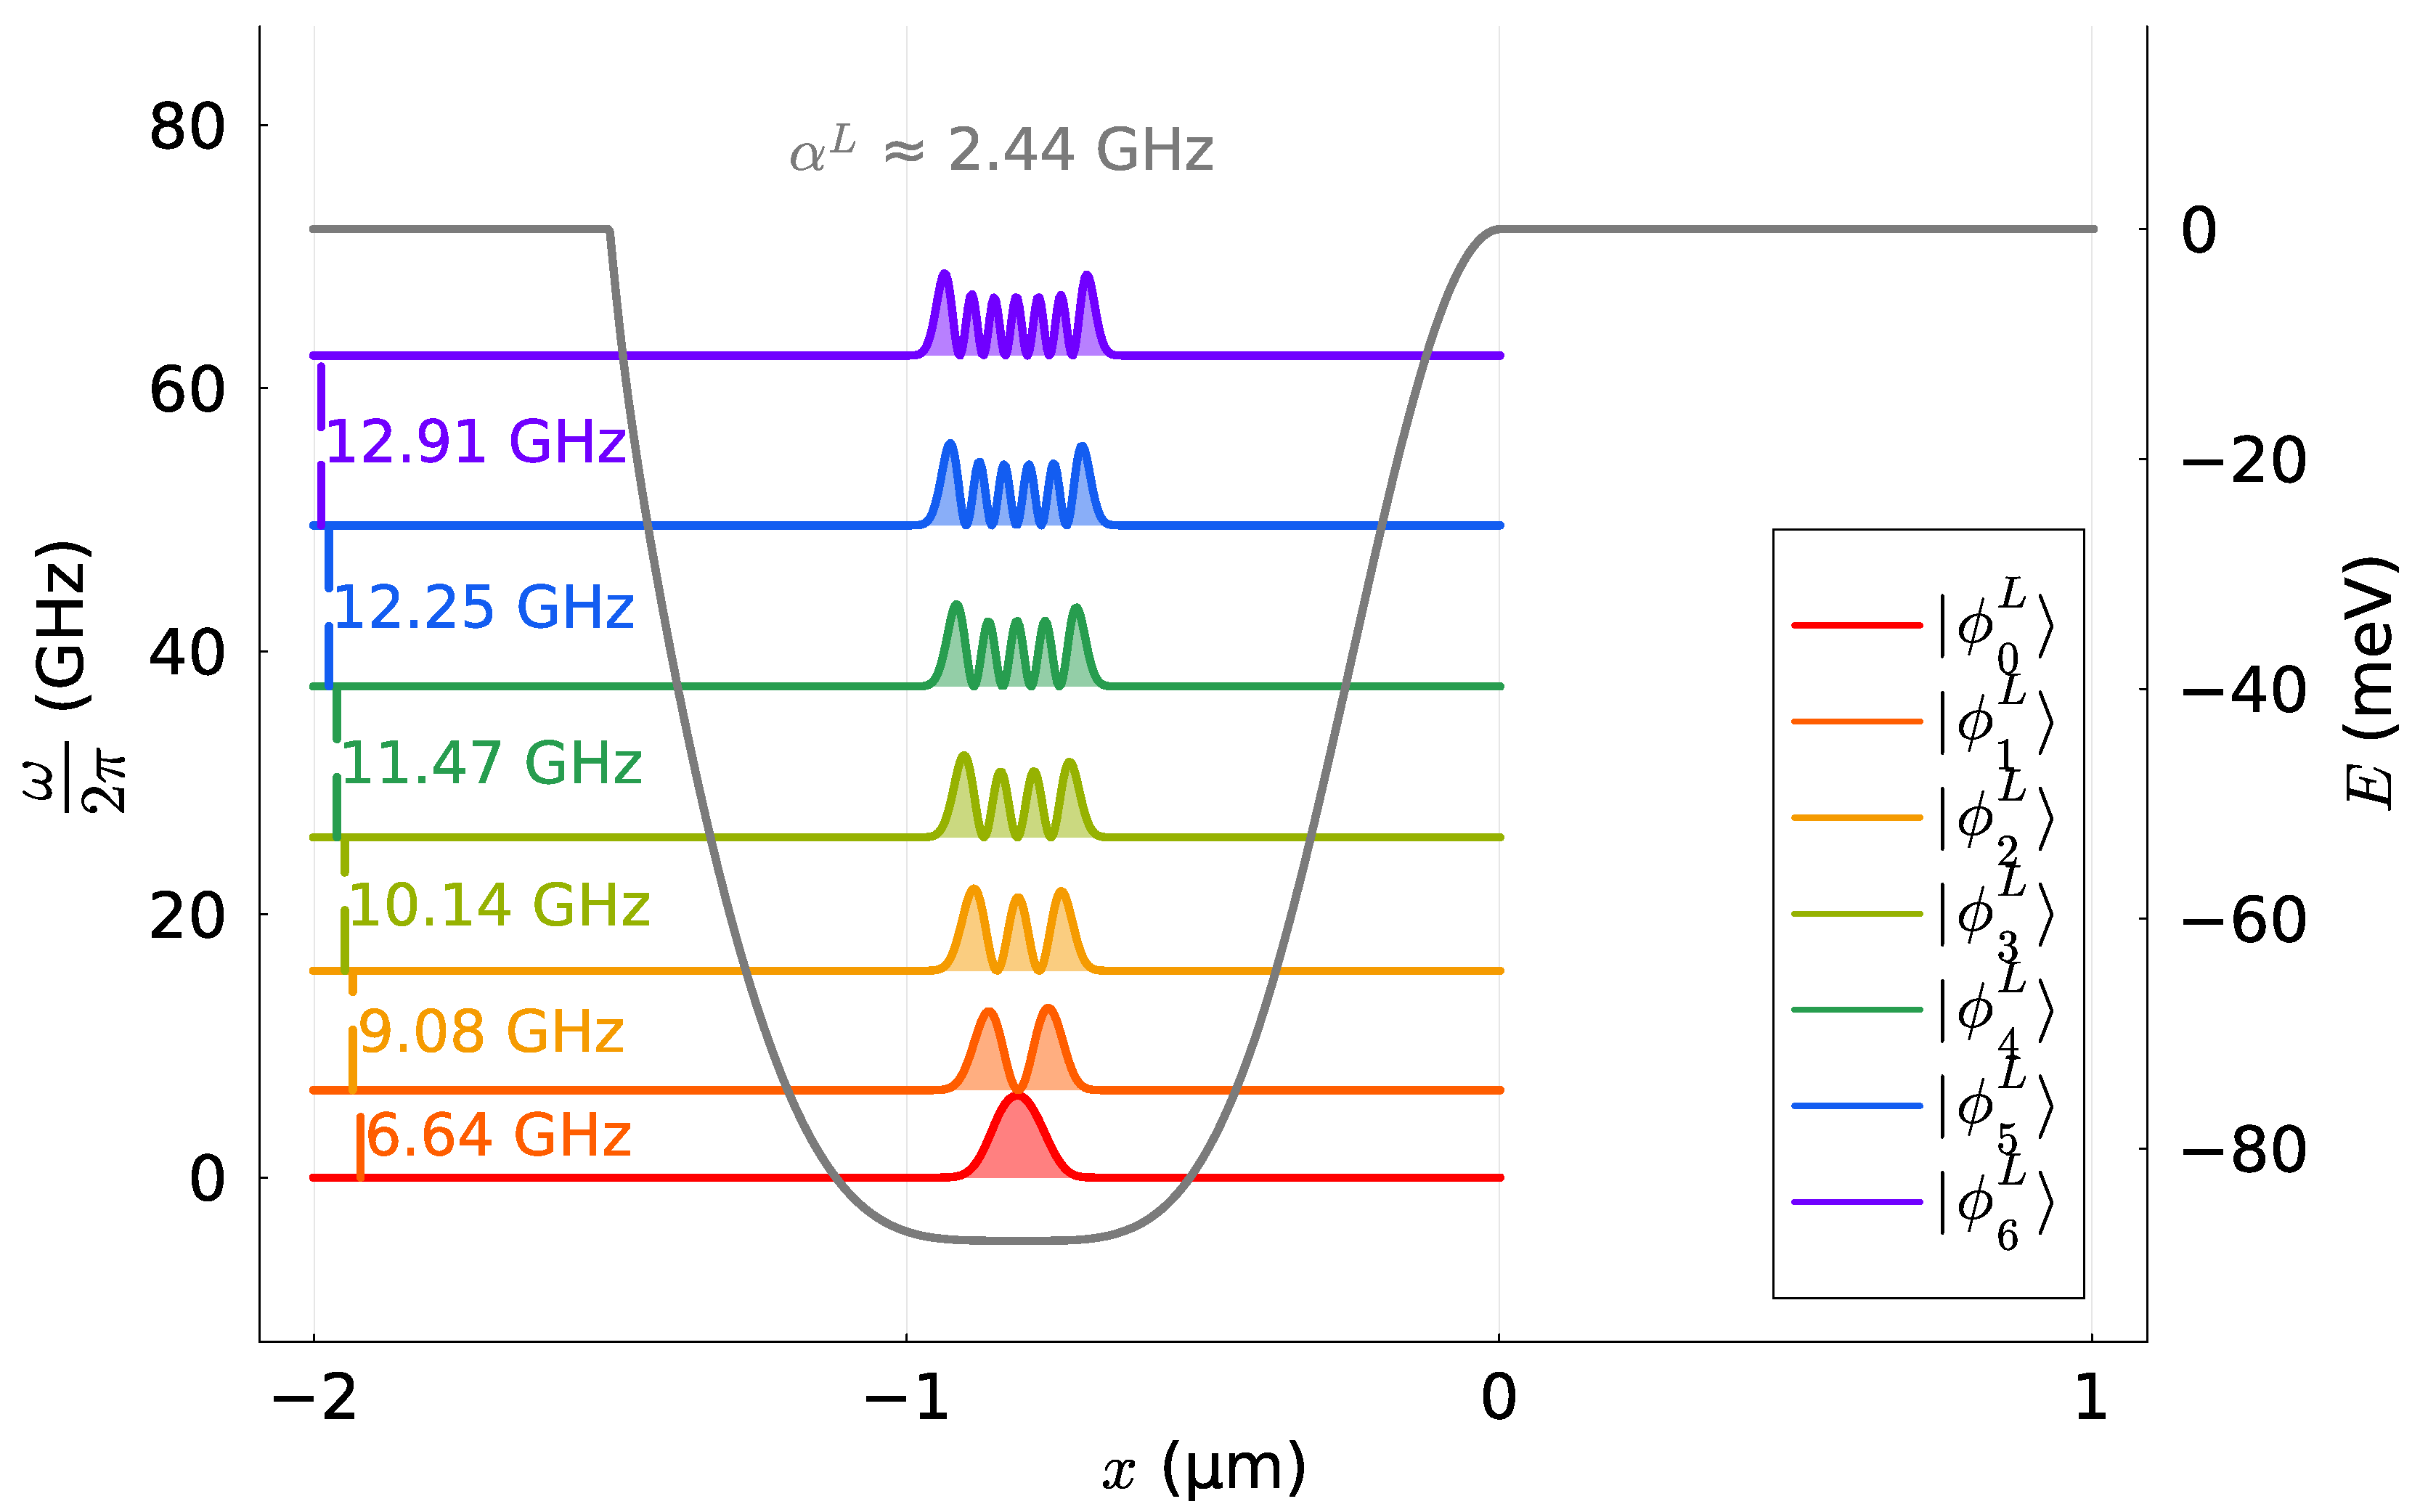
\includegraphics[width=\columnwidth]{figures/figure3_L.pdf}
        \caption{\label{fig:left-basis}The energy basis of the left well in configuration I. %Is this true? 
        Note that the scale differs between the left y-axis, corresponding to the frequencies of the single-particle eigenstates, and the right y-axis, which shows the energy of the potential.
        }
    \end{figure}

    

    \begin{figure}
        \includestandalone[width=\columnwidth]{figures/figuretest}
        \caption{\label{fig:test} A test figure. This figure tests things. We are proud of this figure. (NOTE: This will not be in the final paper. Øyvind is just testing some PGFplots here.)}
    \end{figure}
    Figure \ref{fig:test} is the main result of this work. Read in awe.

    \begin{figure}
        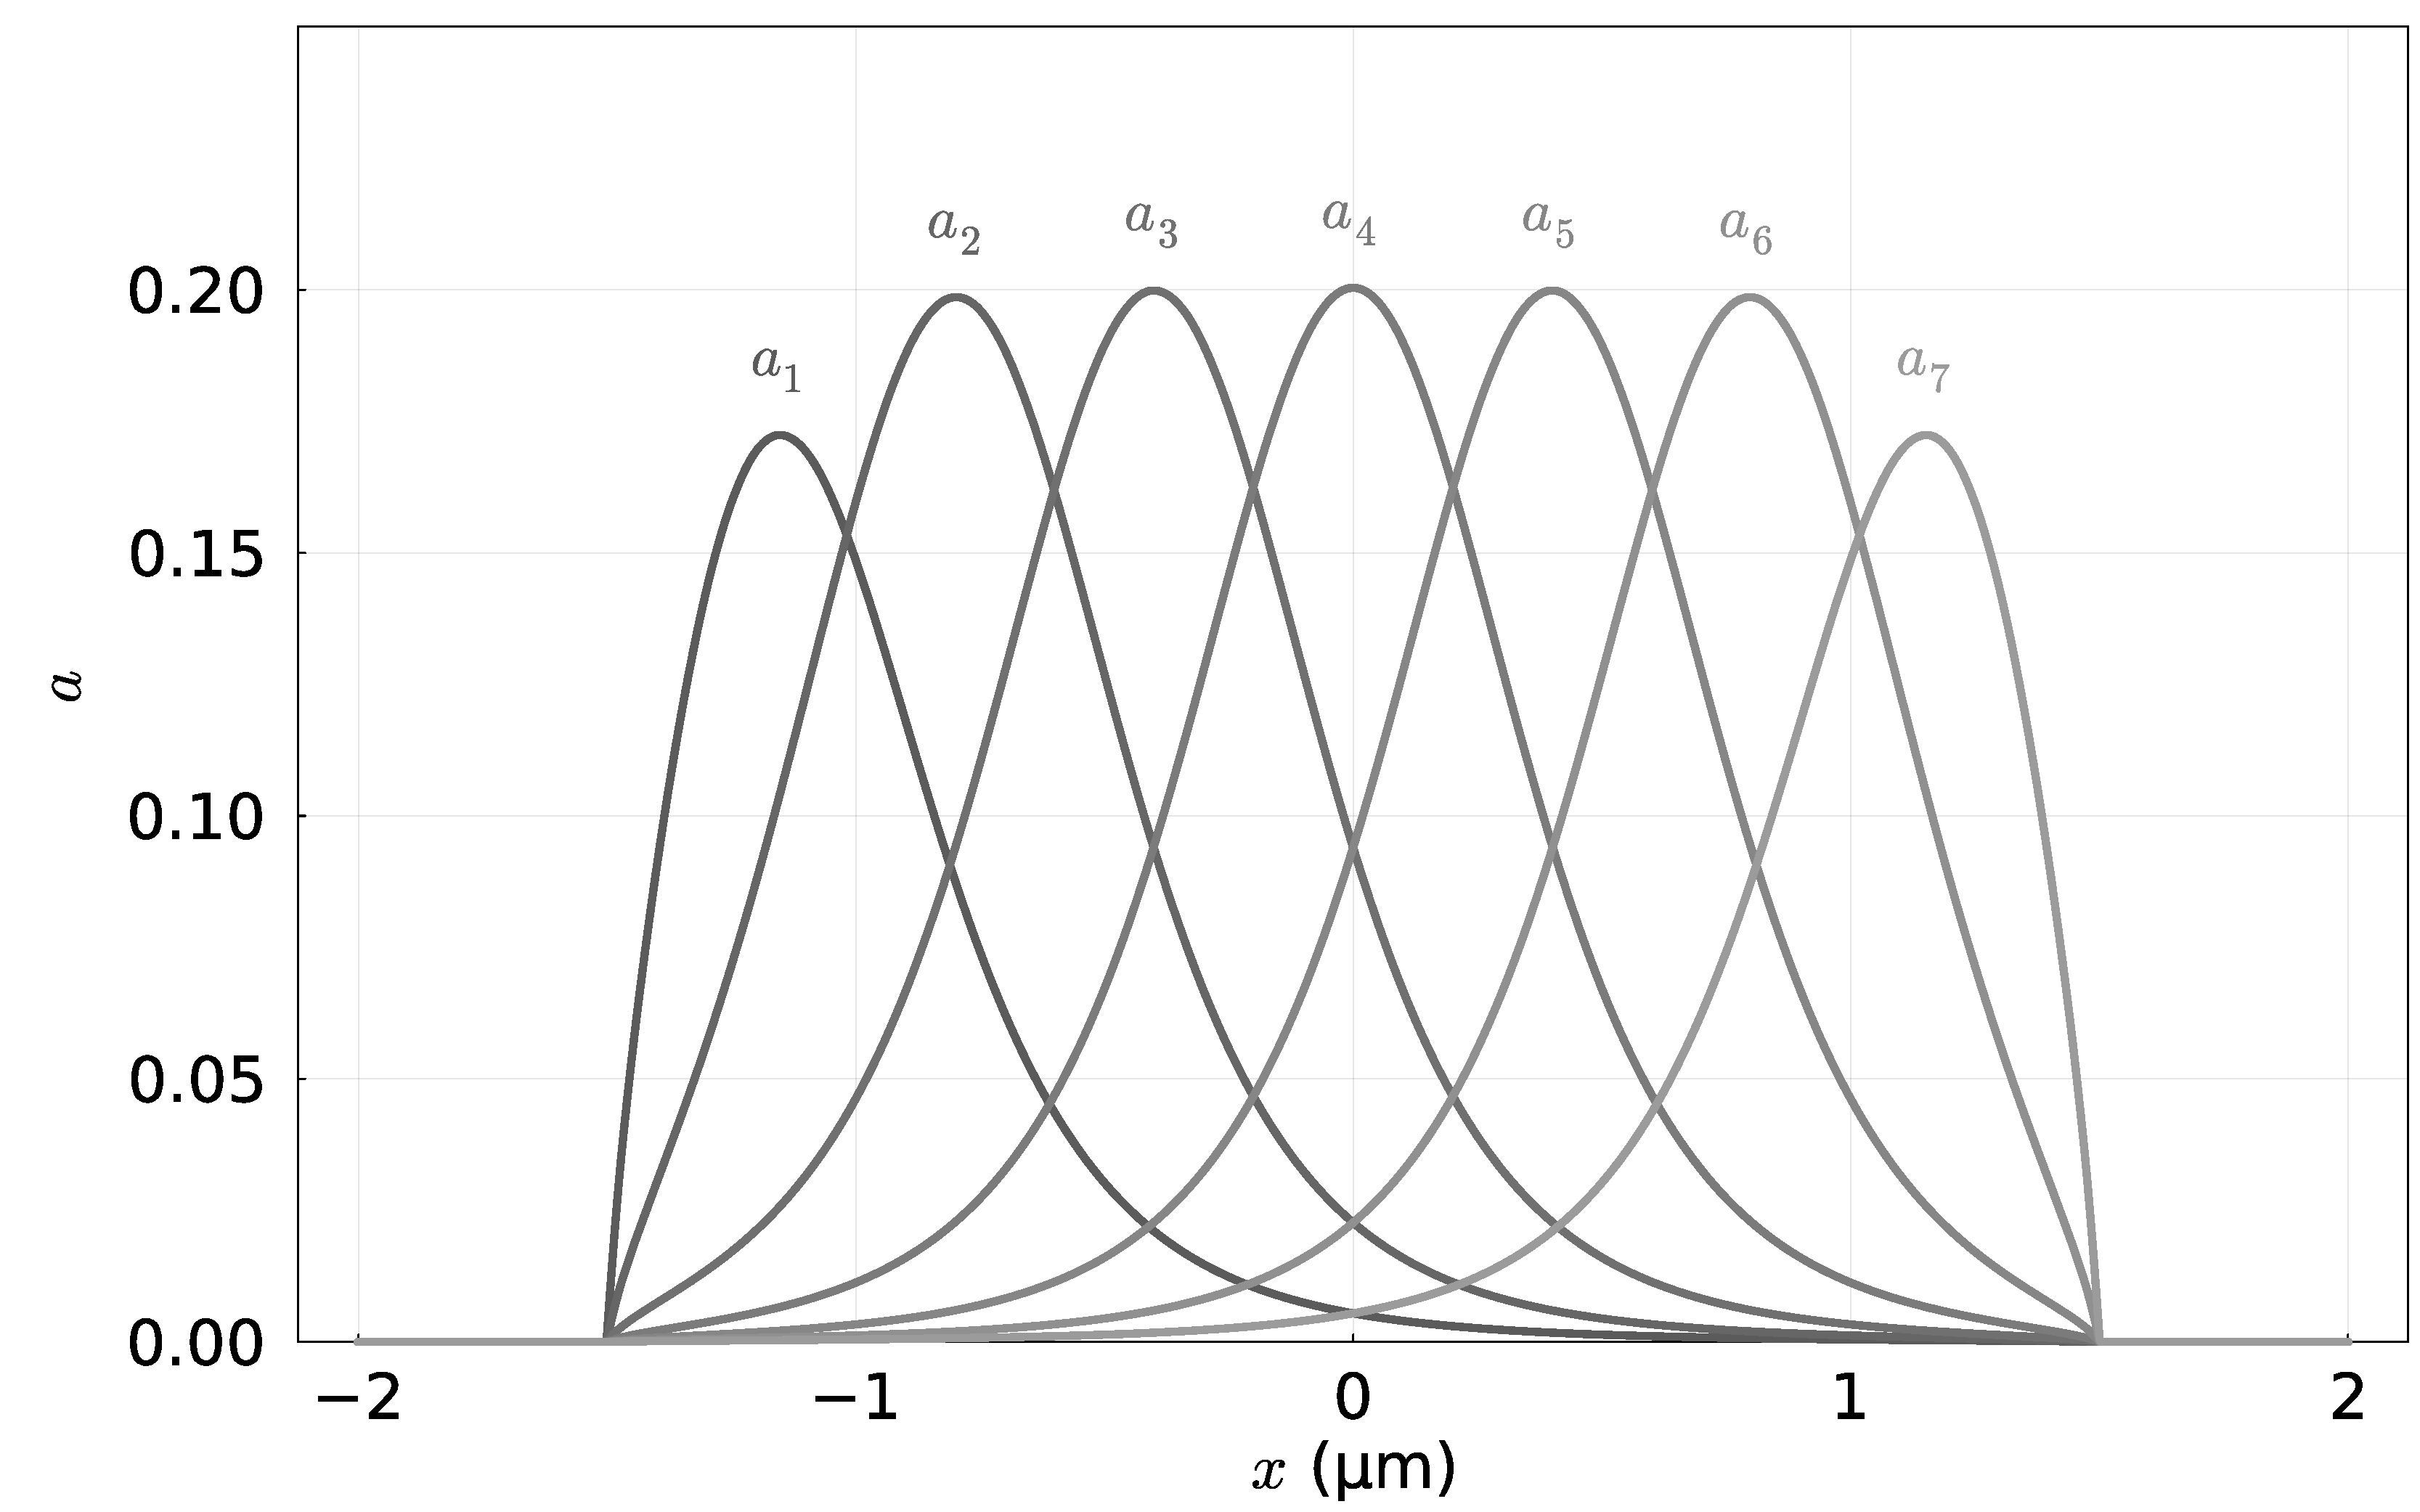
\includegraphics[width=\columnwidth]{figures/figure1_as.pdf}
        \caption{\label{fig:anodes}Anodic basis.}
    \end{figure}

    Using the obtained basis functions, we can proceed to add Coulomb interaction to the system.
    In Fig.~\ref{fig:avoided-crossing} we have plotted the energy spectrum as a function of $\lambda$ for both
    the interacting and the non-interacting case. The right figure clearly shows that the well-parametrization behaves as intended with a clear splitting of the energy levels for $\lambda = 0$, an avoided crossing between $\Psi_1$ and $\Psi_2$ for $\lambda = ?$ and a triple degeneracy point at $\lambda = 1$. %Add label for two figures and label the different configurations? 
    A notable feature of these figures is that the location of the avoided crossings are ``shifted''
    relative to the single-particle crossing points.
    This is a result of the Coulomb interaction not only breaking the degeneracy point seen in the
    single-particle picture, but also altering the potential experienced by the particles. If the potential in the single-particle calculations is modified by adding a point charge in the minima of the opposite well, the energy level crossings coincide with the avoided crossings in the interacting picture.

    \begin{figure}
        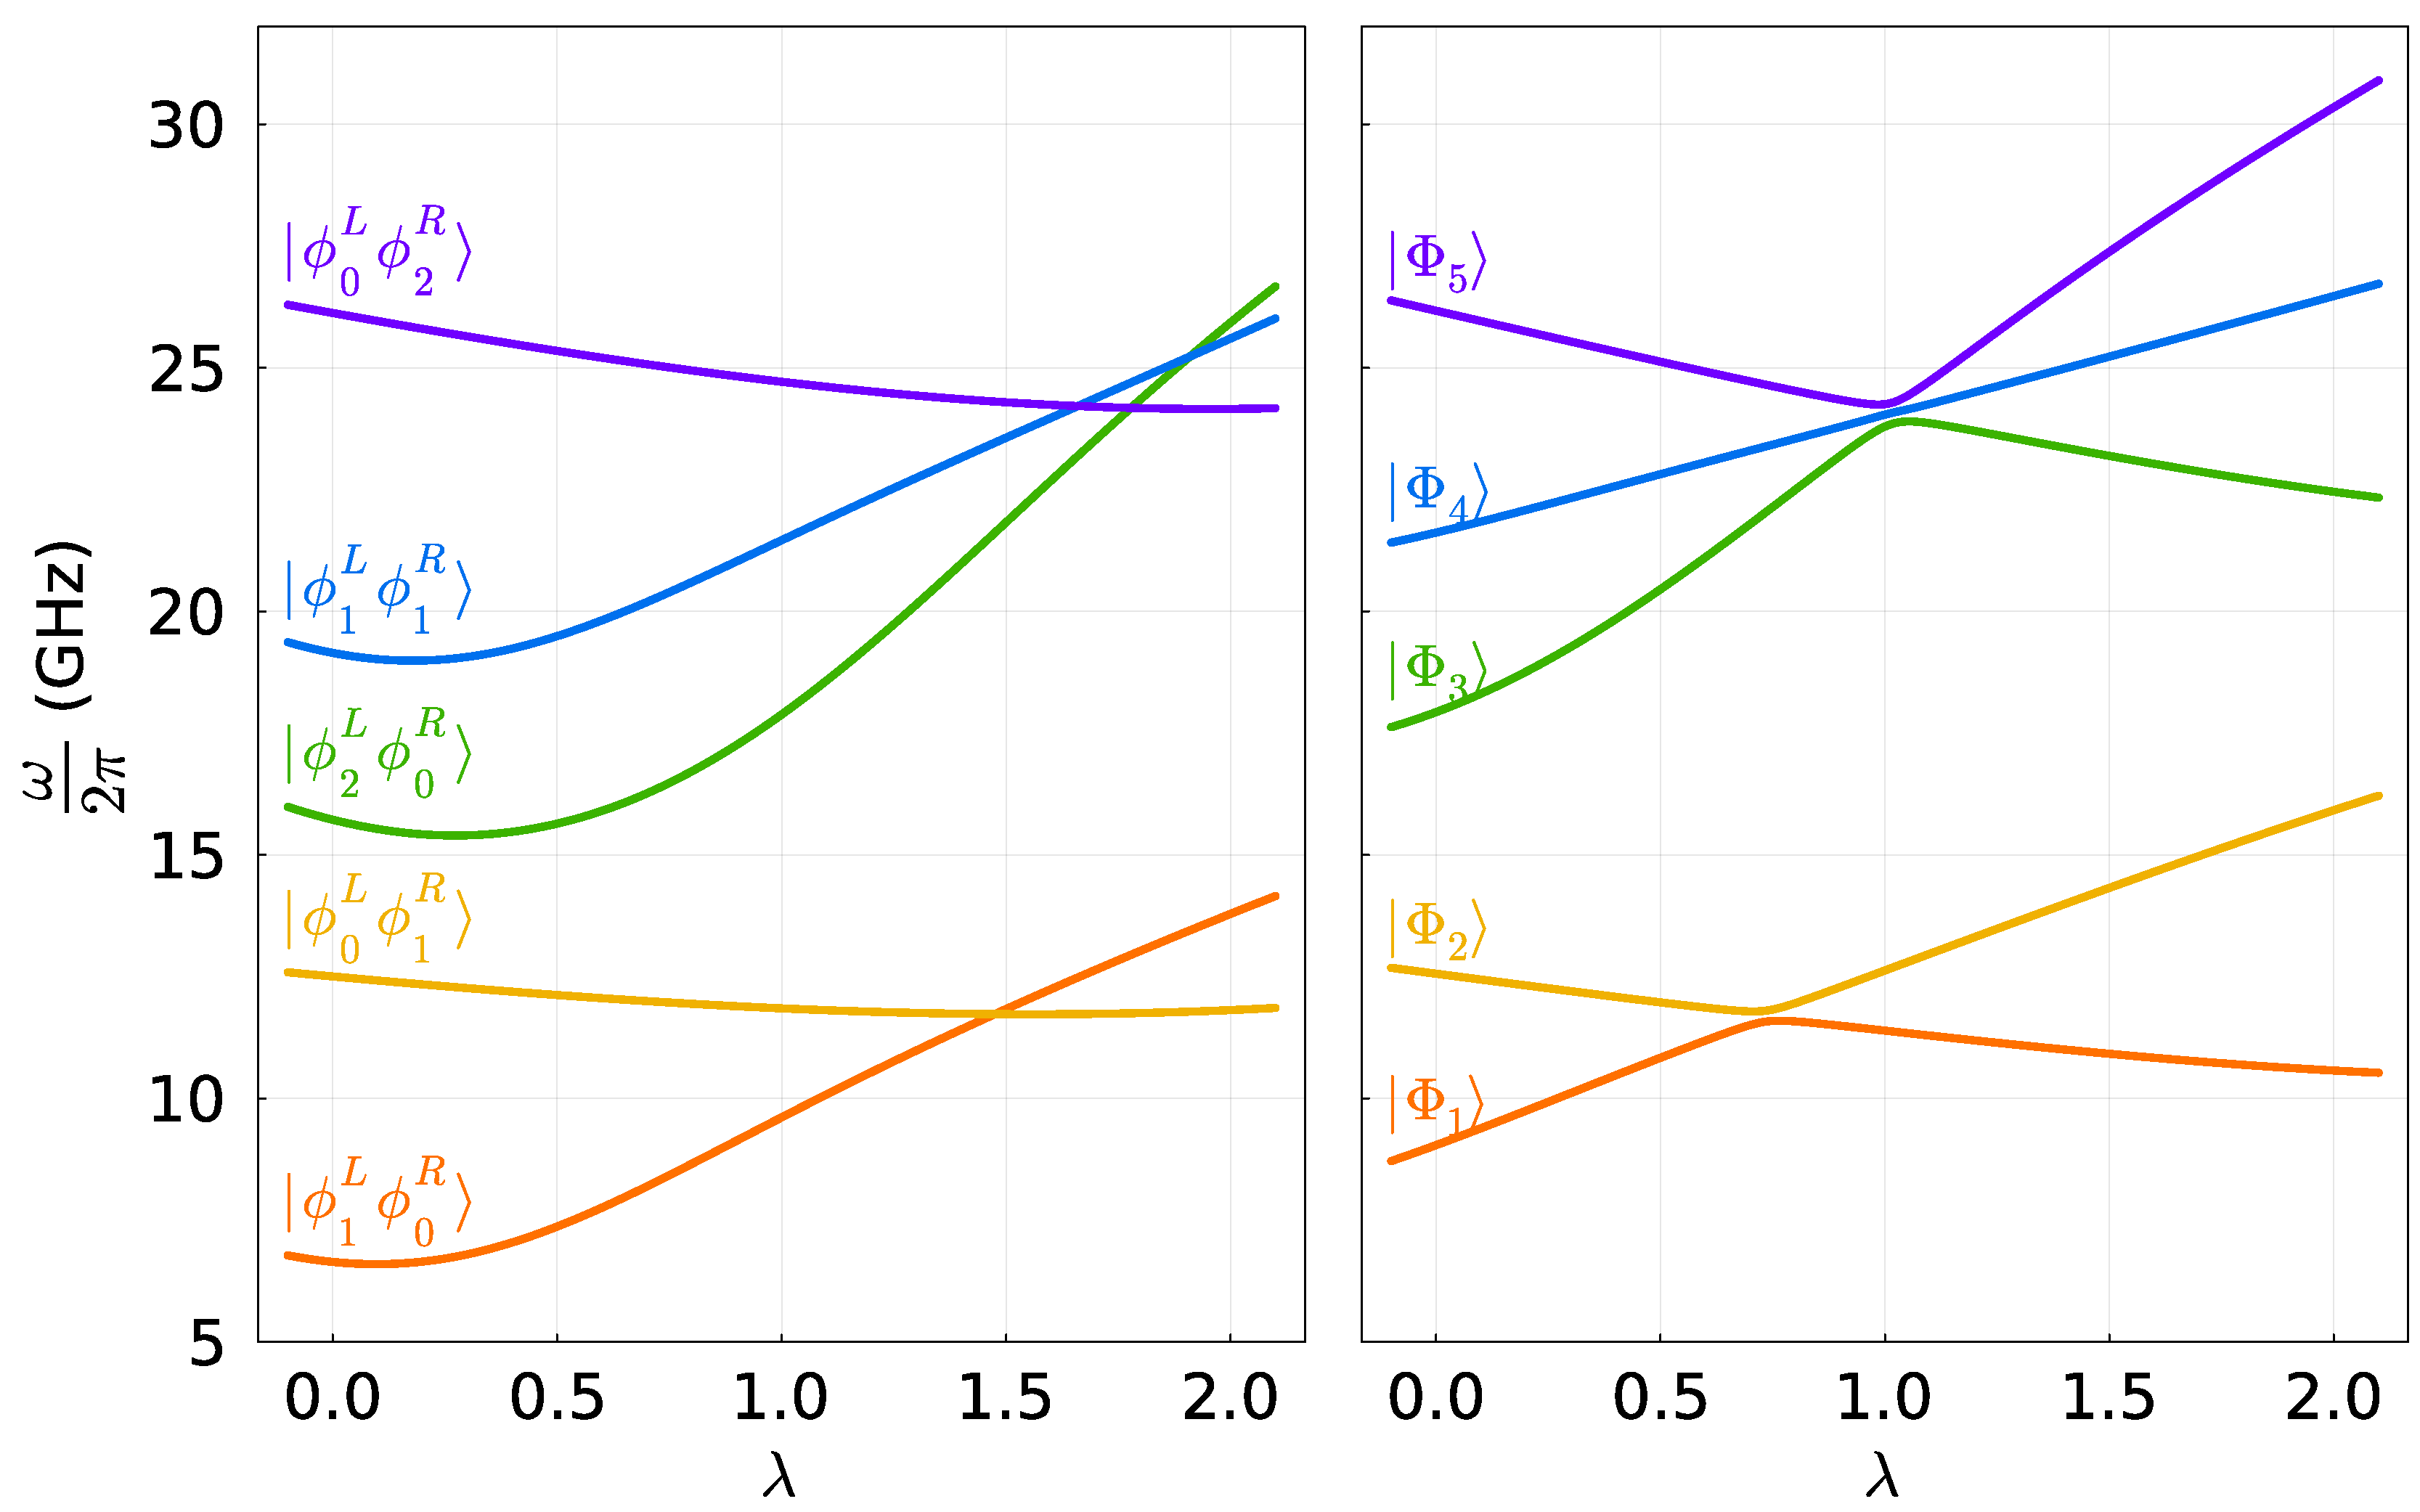
\includegraphics[width=\columnwidth]{figures/figure2.pdf}
        \caption{\label{fig:avoided-crossing}In these figures we have plotted the transition energy from
        the ground state to the labeled excited state as a function of the voltage
        parameter $\lambda$.
        The left figure % TODO: Change to relevant label
        shows the transition energies for the non-interacting case, i.e., the single-particle
        transition energies, whereas the right figure % TODO: Change to relevant label
        shows the interacting situation.}
    \end{figure}


% TODO: various gate description: cross-resonance, c-PHASE gates and estimate the typical 'performance' quantities from final avioded crossing plots 

    % TODO: Consider if we should include Big Chungus, or the split up versions
    % \begin{figure*}
    % 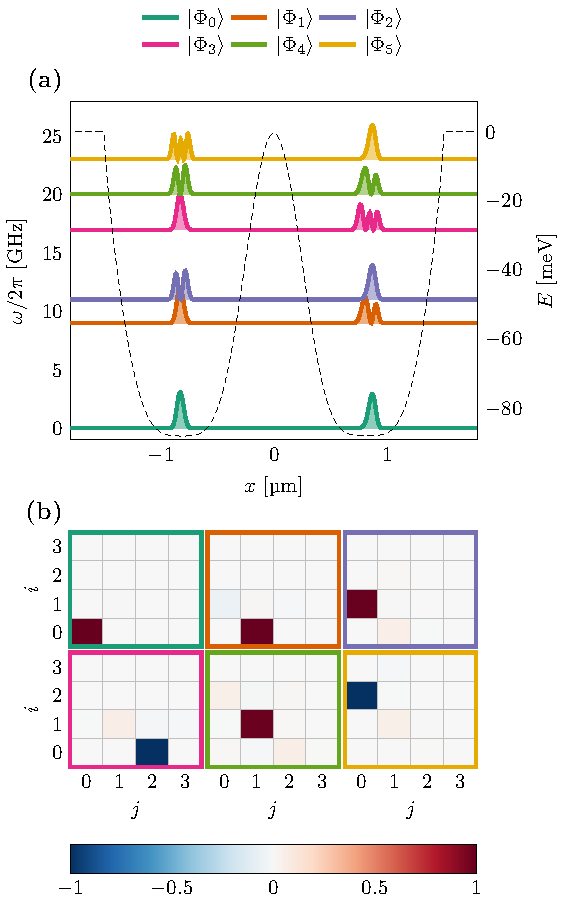
\includegraphics[width=0.99\textwidth]{figures/figure3.pdf}
    % \caption{\label{fig3} (a) Figure caption.}
    % \end{figure*}


In Fig.~\ref{fig:configuration-I} a) %Or whatever we will label it
we can see the potential wells and one-body densities for the measurement configuration, i.e., configuration I described in Sec.~\ref{subsec:ConfigurationI}. The configuration is found by following the procedure explained in Sec.~\ref{sec:opt-well-conf}. We can see that the transition energies for the qubits in the left and right well are within the required frequency range of the set up depicted in Fig.~\ref{fig1}. Each state $\ket{\Phi_i}$ is a linear combination of the basis functions, with coefficients depicted in fig.~\ref{fig:configuration-I} b). The figure shows that every state has several components in the basis constructed from the single-particle eigenstates, which makes it unsuitable as a computational basis. We instead define the computational basis by the Schmidt decomposition as described in section~\ref{subsec:computational-basis}. The active single-particle states in the Schmidt basis are plotted in fig.~\ref{fig:configuration-I} c). The ideal configuration should include only one active single-particle state in the Schmidt basis as this would imply that the corresponding state can be written as a product state, and there is hence no entanglement between the qubits. We see in the heat maps that there is one dominating state for every energy level, however some of the energy levels have a non-zero amplitude for more than one single-particle state.
% Some discussion on how to quantify the error due to the states not being perfect product-states?

    \begin{figure}
        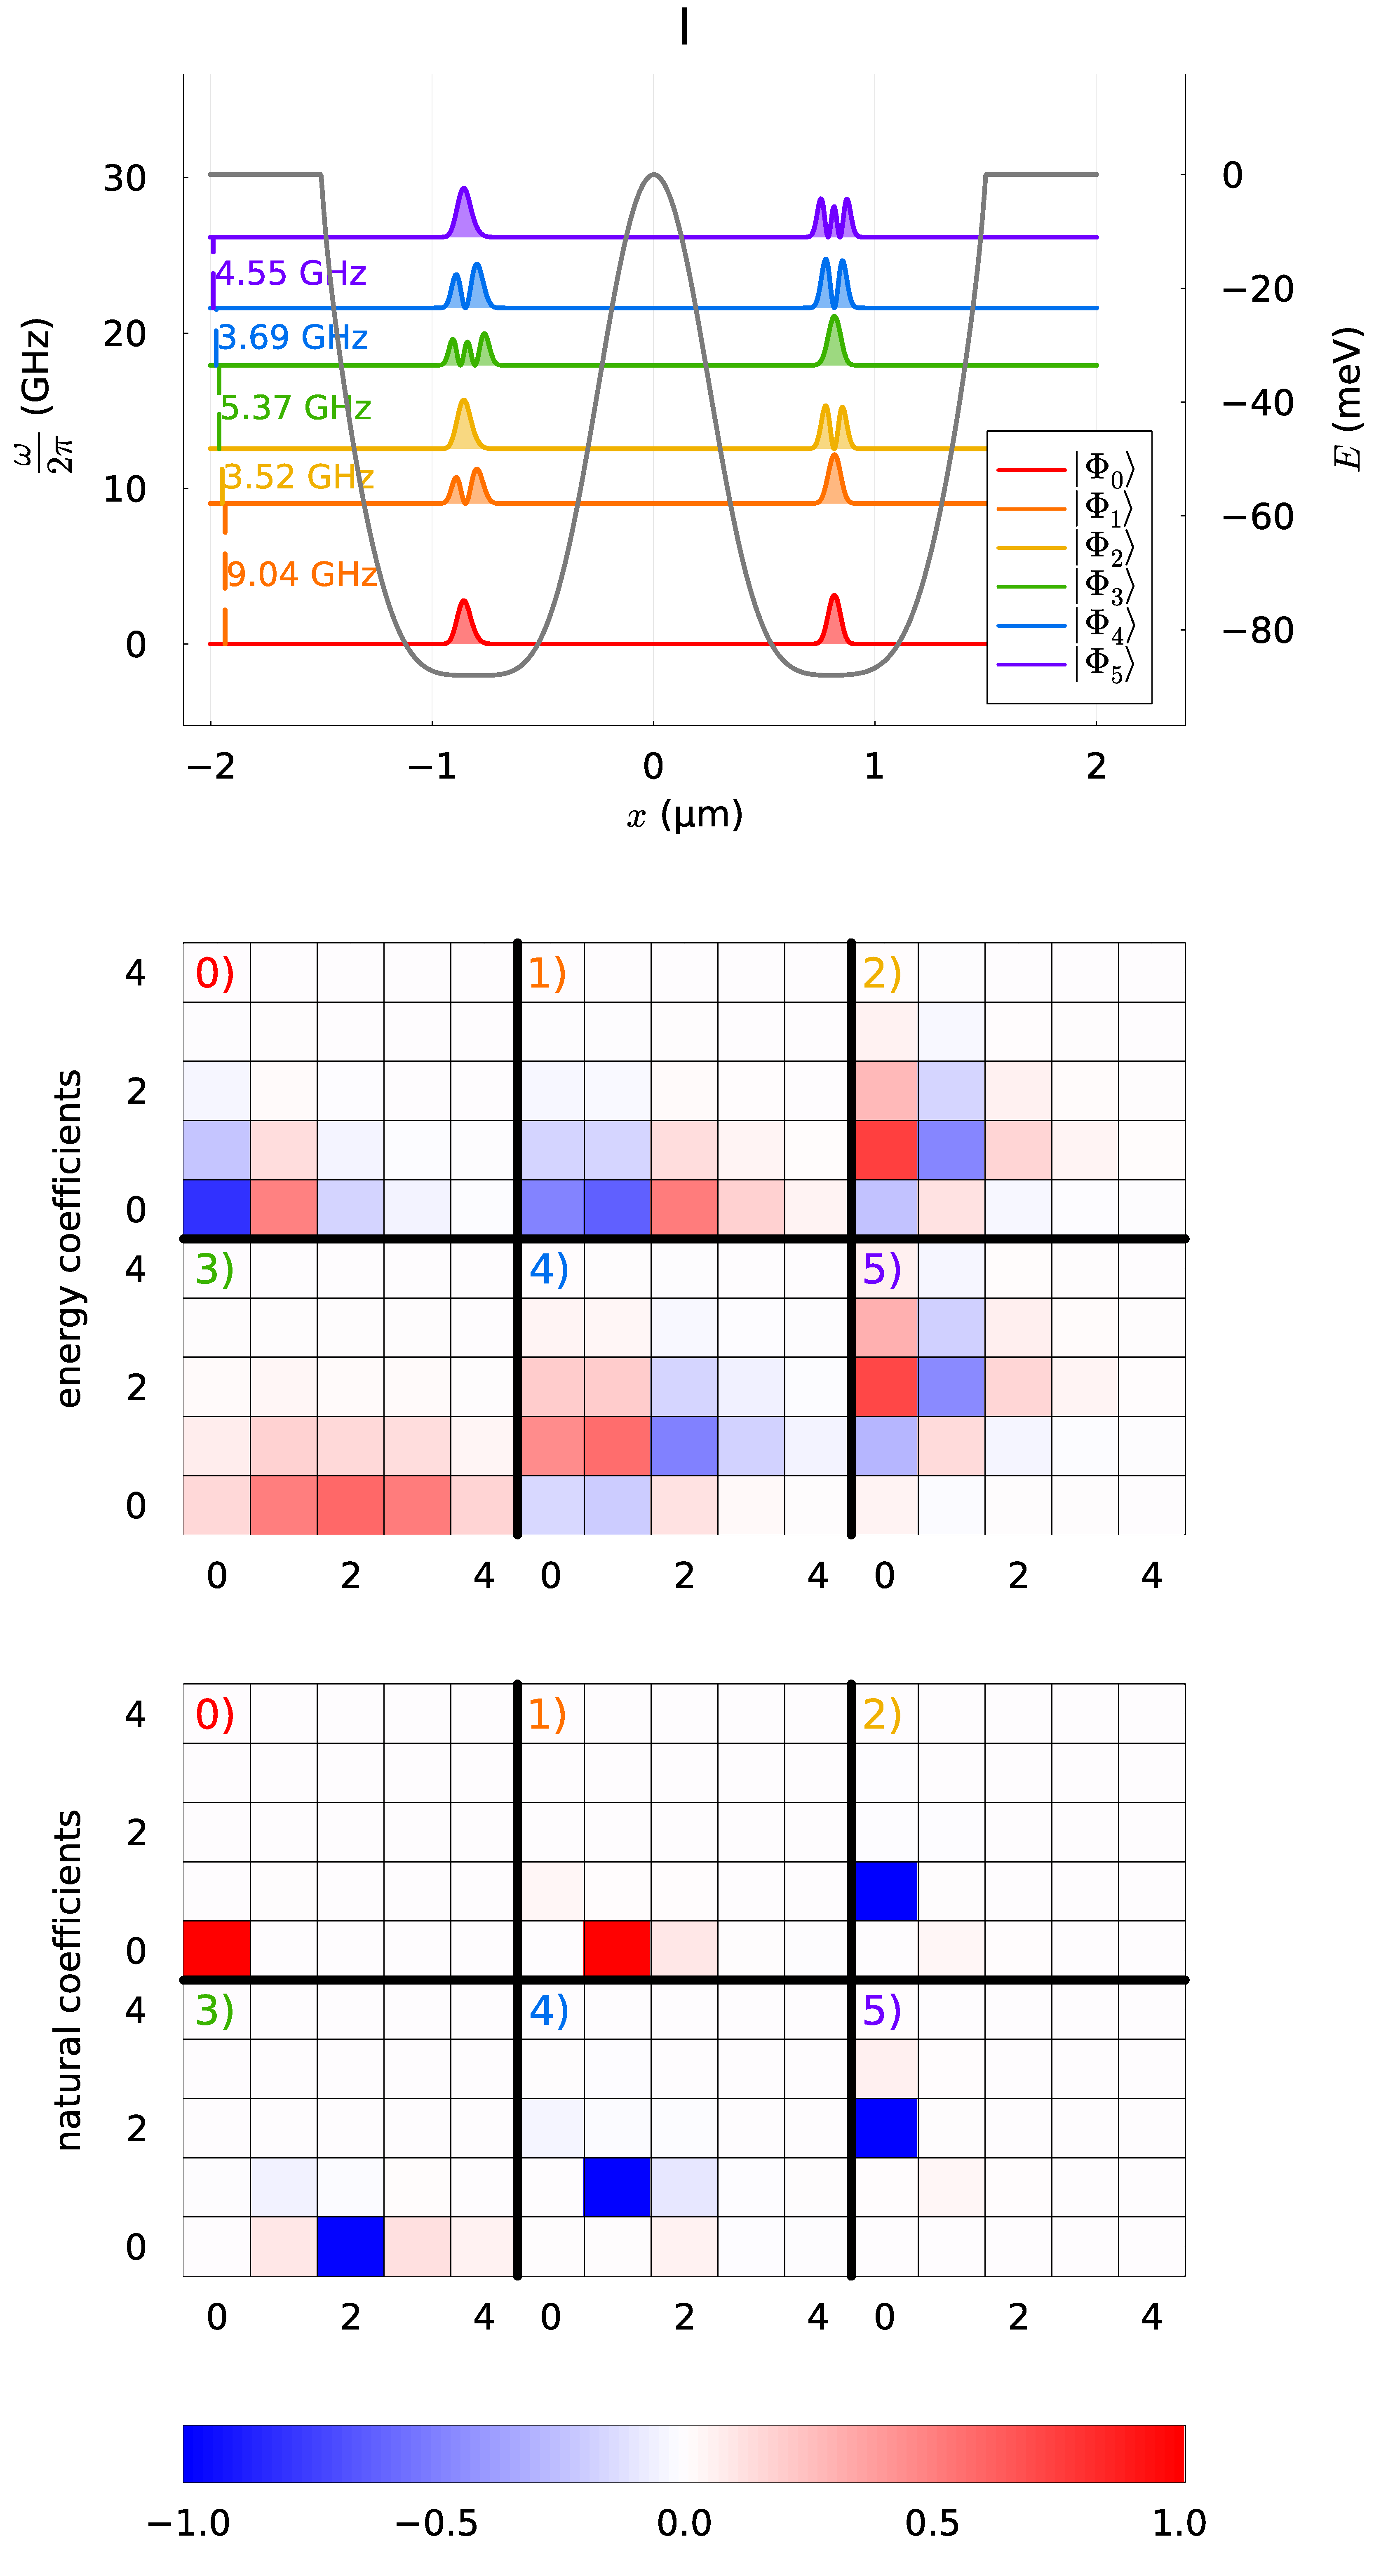
\includegraphics[width=\columnwidth]{figures/figure3_Ib_full.pdf}
        \caption{\label{fig:configuration-I}These figures depict the potential wells, the one-body
        densities, and the active single-particle states in the Schmidt basis for configuration I,
        i.e., in the measurement regime.
        In the topmost figure % TODO: Add label
        we have plotted the potential wells for electrode voltages
        $\vb{V}_{\mathrm{I}}$ (the right-axis reflects the potential energy), and the one-body
        densities added to the transition energies of each state (left-axis gives the
        transition energies).
        The middle figure %TODO: Add label
        shows the coefficients in the basis consisting of the single-particle eigenstates, with plot n) depicting the coefficients of $\ket*{\Phi_n}$. The square labeled by $i$($j$) on the x(y)-axis corresponds to the coefficient in front of the $\ket*{\phi_i^L\phi_j^R}$ component. 
        The bottom figure % TODO: Add label
        shows the coefficients in the computational basis obtained by performing a Schmidt decomposition of the ground state. The plot is read in the same way as plot b). Note that $\ket*{\Phi_0}$ by construction only has a $\ket*{\psi^L_0\psi^R_0}$ component. All other states also have one dominating component, but some other non-zero coefficients can be seen for instance in the $\ket*{\Phi_3}$ state.  
        % Not sure about the titles left of the figures here, they can be misinterpreted as y-labels.
        }
    \end{figure}

In Fig.~\ref{fig3_II} we can see the one-body densities and the active single-particle states for configuration II and III. The plots for configuration II show how the $\ket*{\Phi_1}$ and $\ket*{\Phi_2}$ states no longer can be expressed as product states, but instead become linear combinations 
\begin{align*}
    \ket*{\Phi_1} &= \frac{-1}{\sqrt{2}}\left(\ket{\psi_0^L\psi_1^R}+\ket{\psi_1^L\psi_0^R}\right)\\
    \ket*{\Phi_2} &= \frac{1}{\sqrt{2}}\left(\ket{\psi_0^L\psi_1^R}-\ket{\psi_1^L\psi_0^R}\right),
\end{align*}
 where the global phase factor -1 in $\ket*{\Phi_1}$ is included for agreement with the color coding of the plot. The higher eigenstates are still fairly well described by product states, which should make this configuration possible to use for an entangling gate without too much leakage. We get similar results for configuration III, where the $\ket*{\Phi_3}$, $\ket*{\Phi_4}$ and $\ket*{\Phi_5}$ states become linear combinations whereas the $\ket*{\Phi_1}$ and $\ket*{\Phi_2}$ are well approximated by product states. This should make configuration III suitable for controlled phase gates with low swap error.

\begin{figure*}
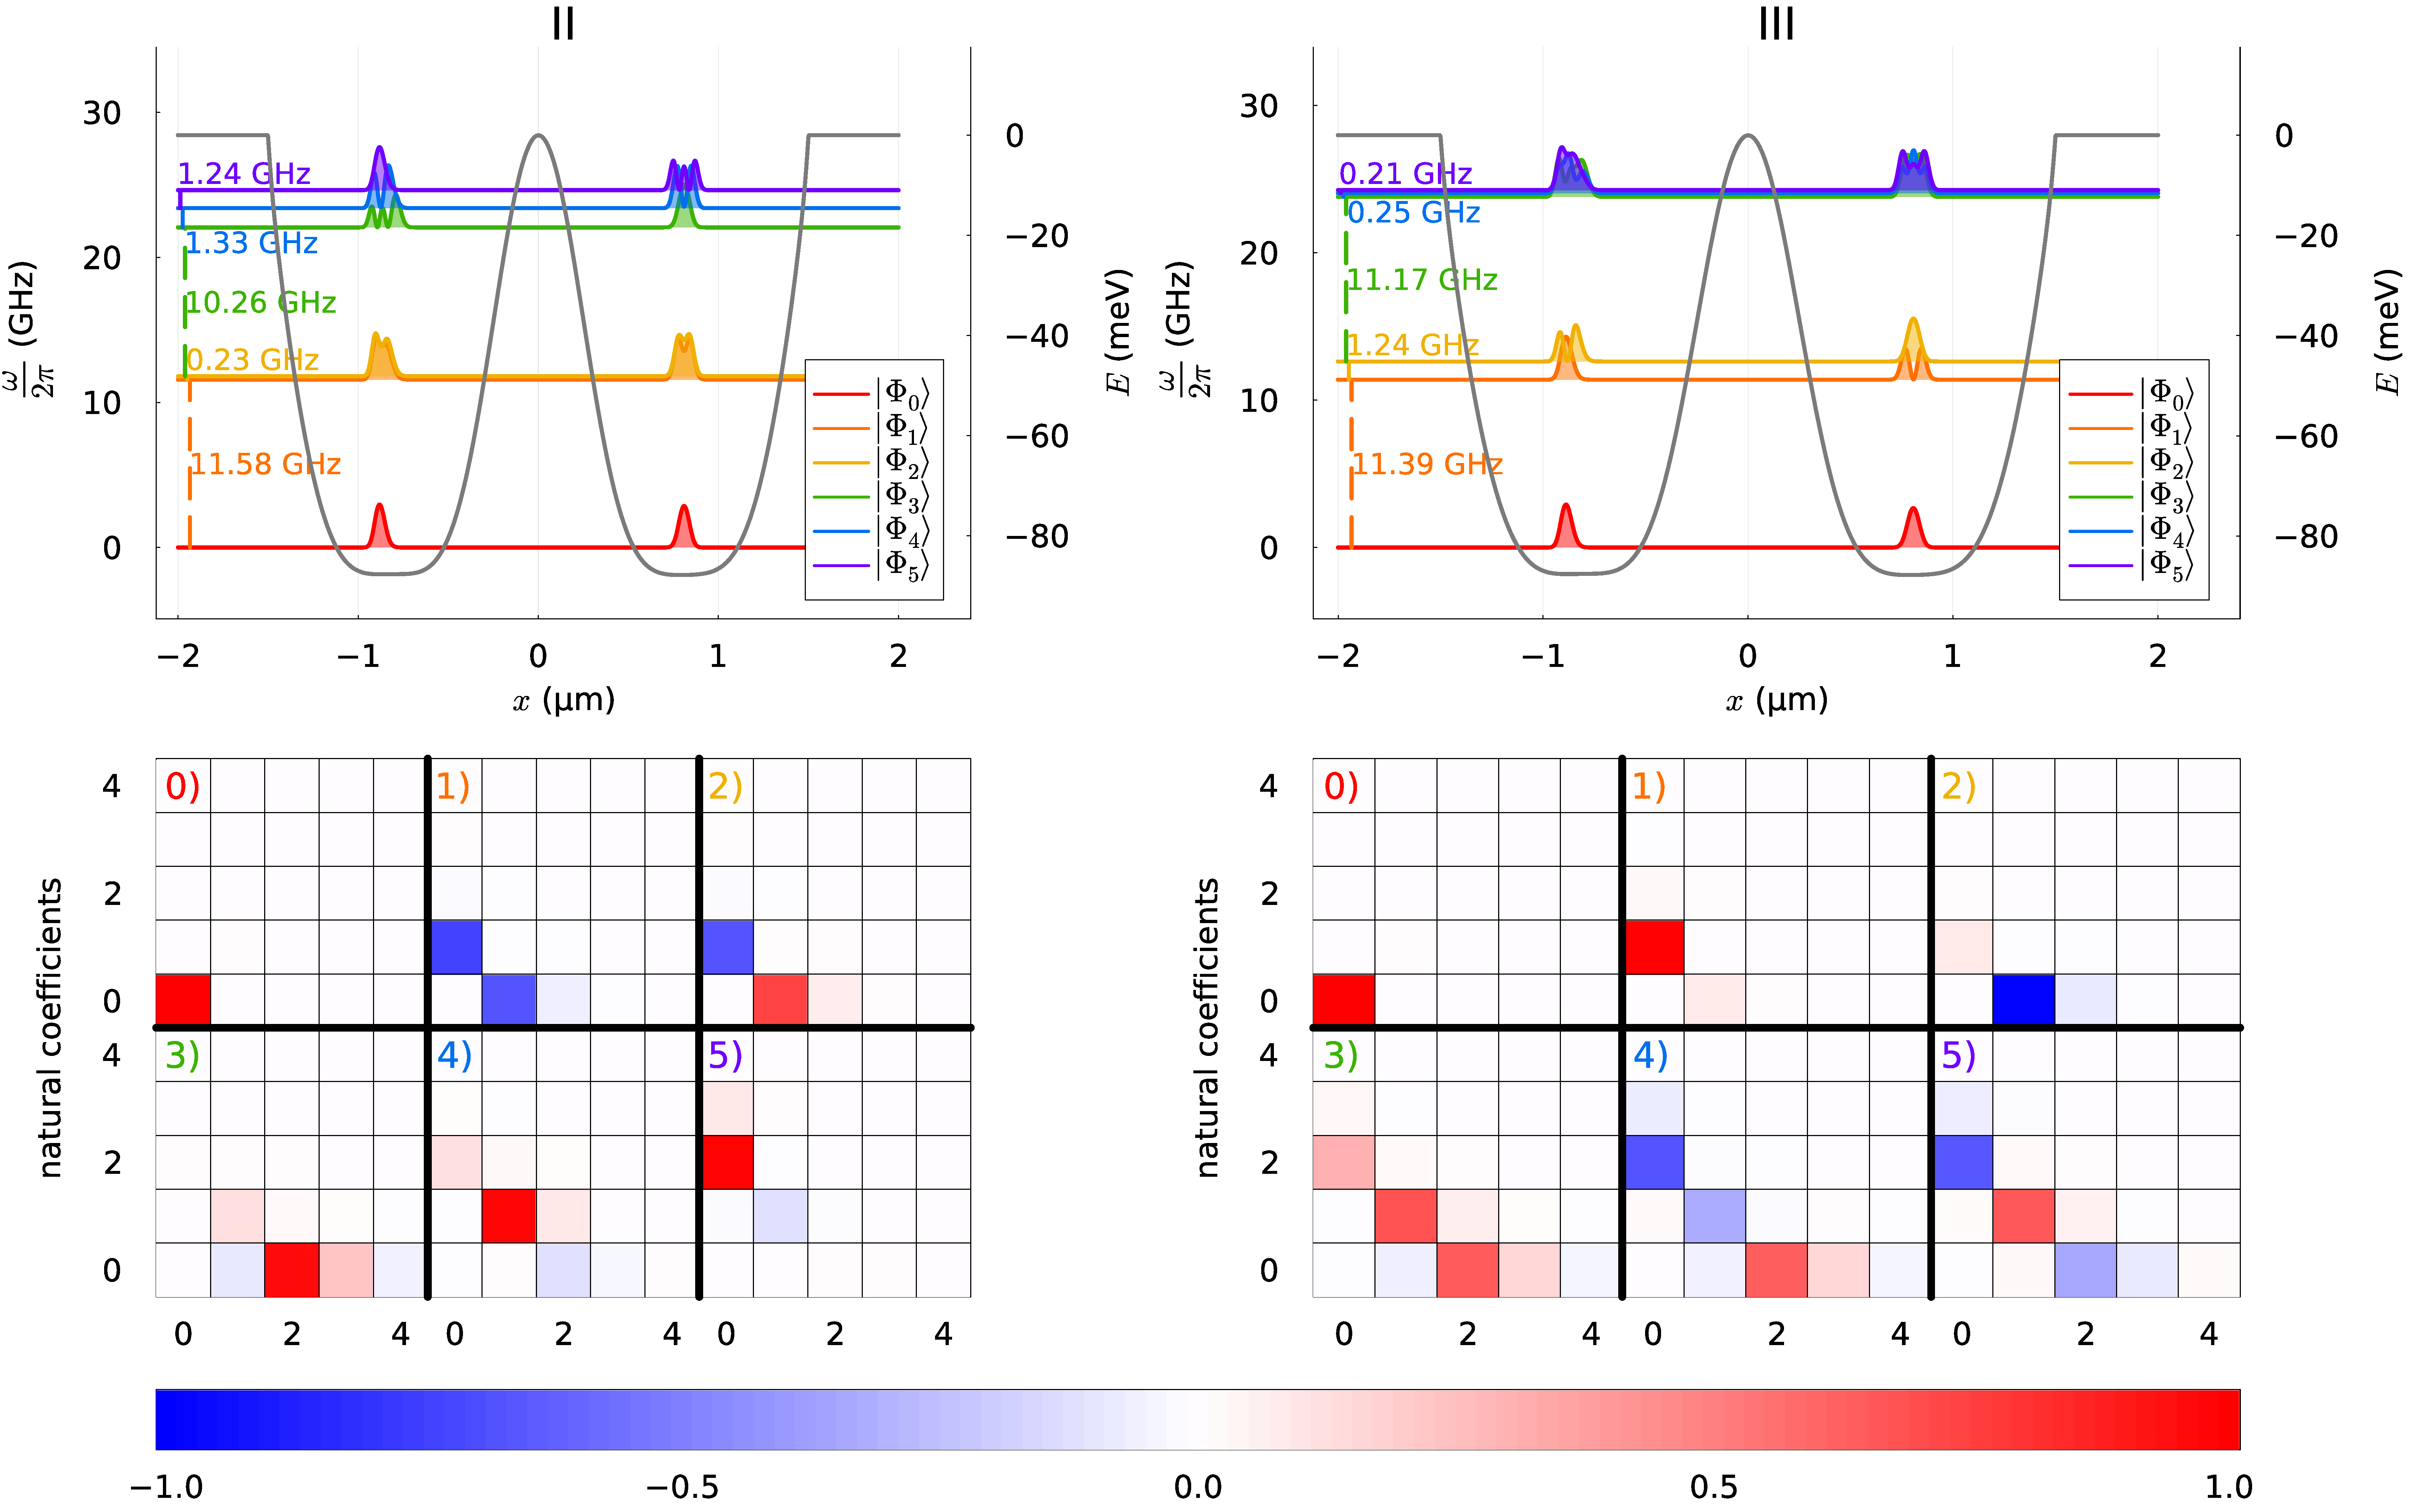
\includegraphics[width=0.99\textwidth]{figures/figure3_II_IIIb.pdf}
\caption{\label{fig3_II} These figures depict the potential wells, the one-body
        densities, and the active single-particle states in the Schmidt basis for configurations II and III,
        i.e., in the avoided crossing regimes.
        In the topmost figures % TODO: Add label
        we have plotted the potential wells for electrode voltages
        $\vb{V}_{\mathrm{II}}$ and $\vb{V}_{\mathrm{III}}$ (the right-axis reflects the potential energy), and the one-body
        densities added to the transition energies of each state (left-axis gives the
        transition energies).
        The bottom figures % TODO: Add label
        shows the coefficients in the Schmidt basis, with plot n) depicting the coefficients of $\ket*{\Phi_n}$. The square labeled by $i$($j$) on the x(y)-axis corresponds to the coefficient in front of the $\ket*{\psi_i^L\psi_j^R}$ component. }
\end{figure*}

% TODO: Plot the entropy as a function of the well
% configurations.

    The interaction between the computational basis states can be characterized by the von Neumann entropy, which is plotted as a function of voltage parameter $\lambda$ in fig.~\ref{fig:entropies}. We see from the figure that we are able to transition from the detuned configuration I ($\lambda = 0$) to the avoided crossing of configuration II ($\lambda = ?$) and configuration III ($\lambda = 1$) by adiabatically adjusting the voltage parameter. For configuration II (III), we would ideally only want the entropies $S_1$ and $S_2$ ($S_3$, $S_4$ and $S_5$) to be non-zero as this would ensure that no leakage occur to unwanted states while transitioning to the different configurations. We do not achieve the ideal behaviour in this example, but we expect that this can be improved by adding more nodes or adjusting the spatial separation between the nodes. This would in turn allow more flexibility in adjusting the well shapes or allow a larger separation between each well and hence decrease the coloumb-interaction between the electrons.

    \begin{figure}
        % 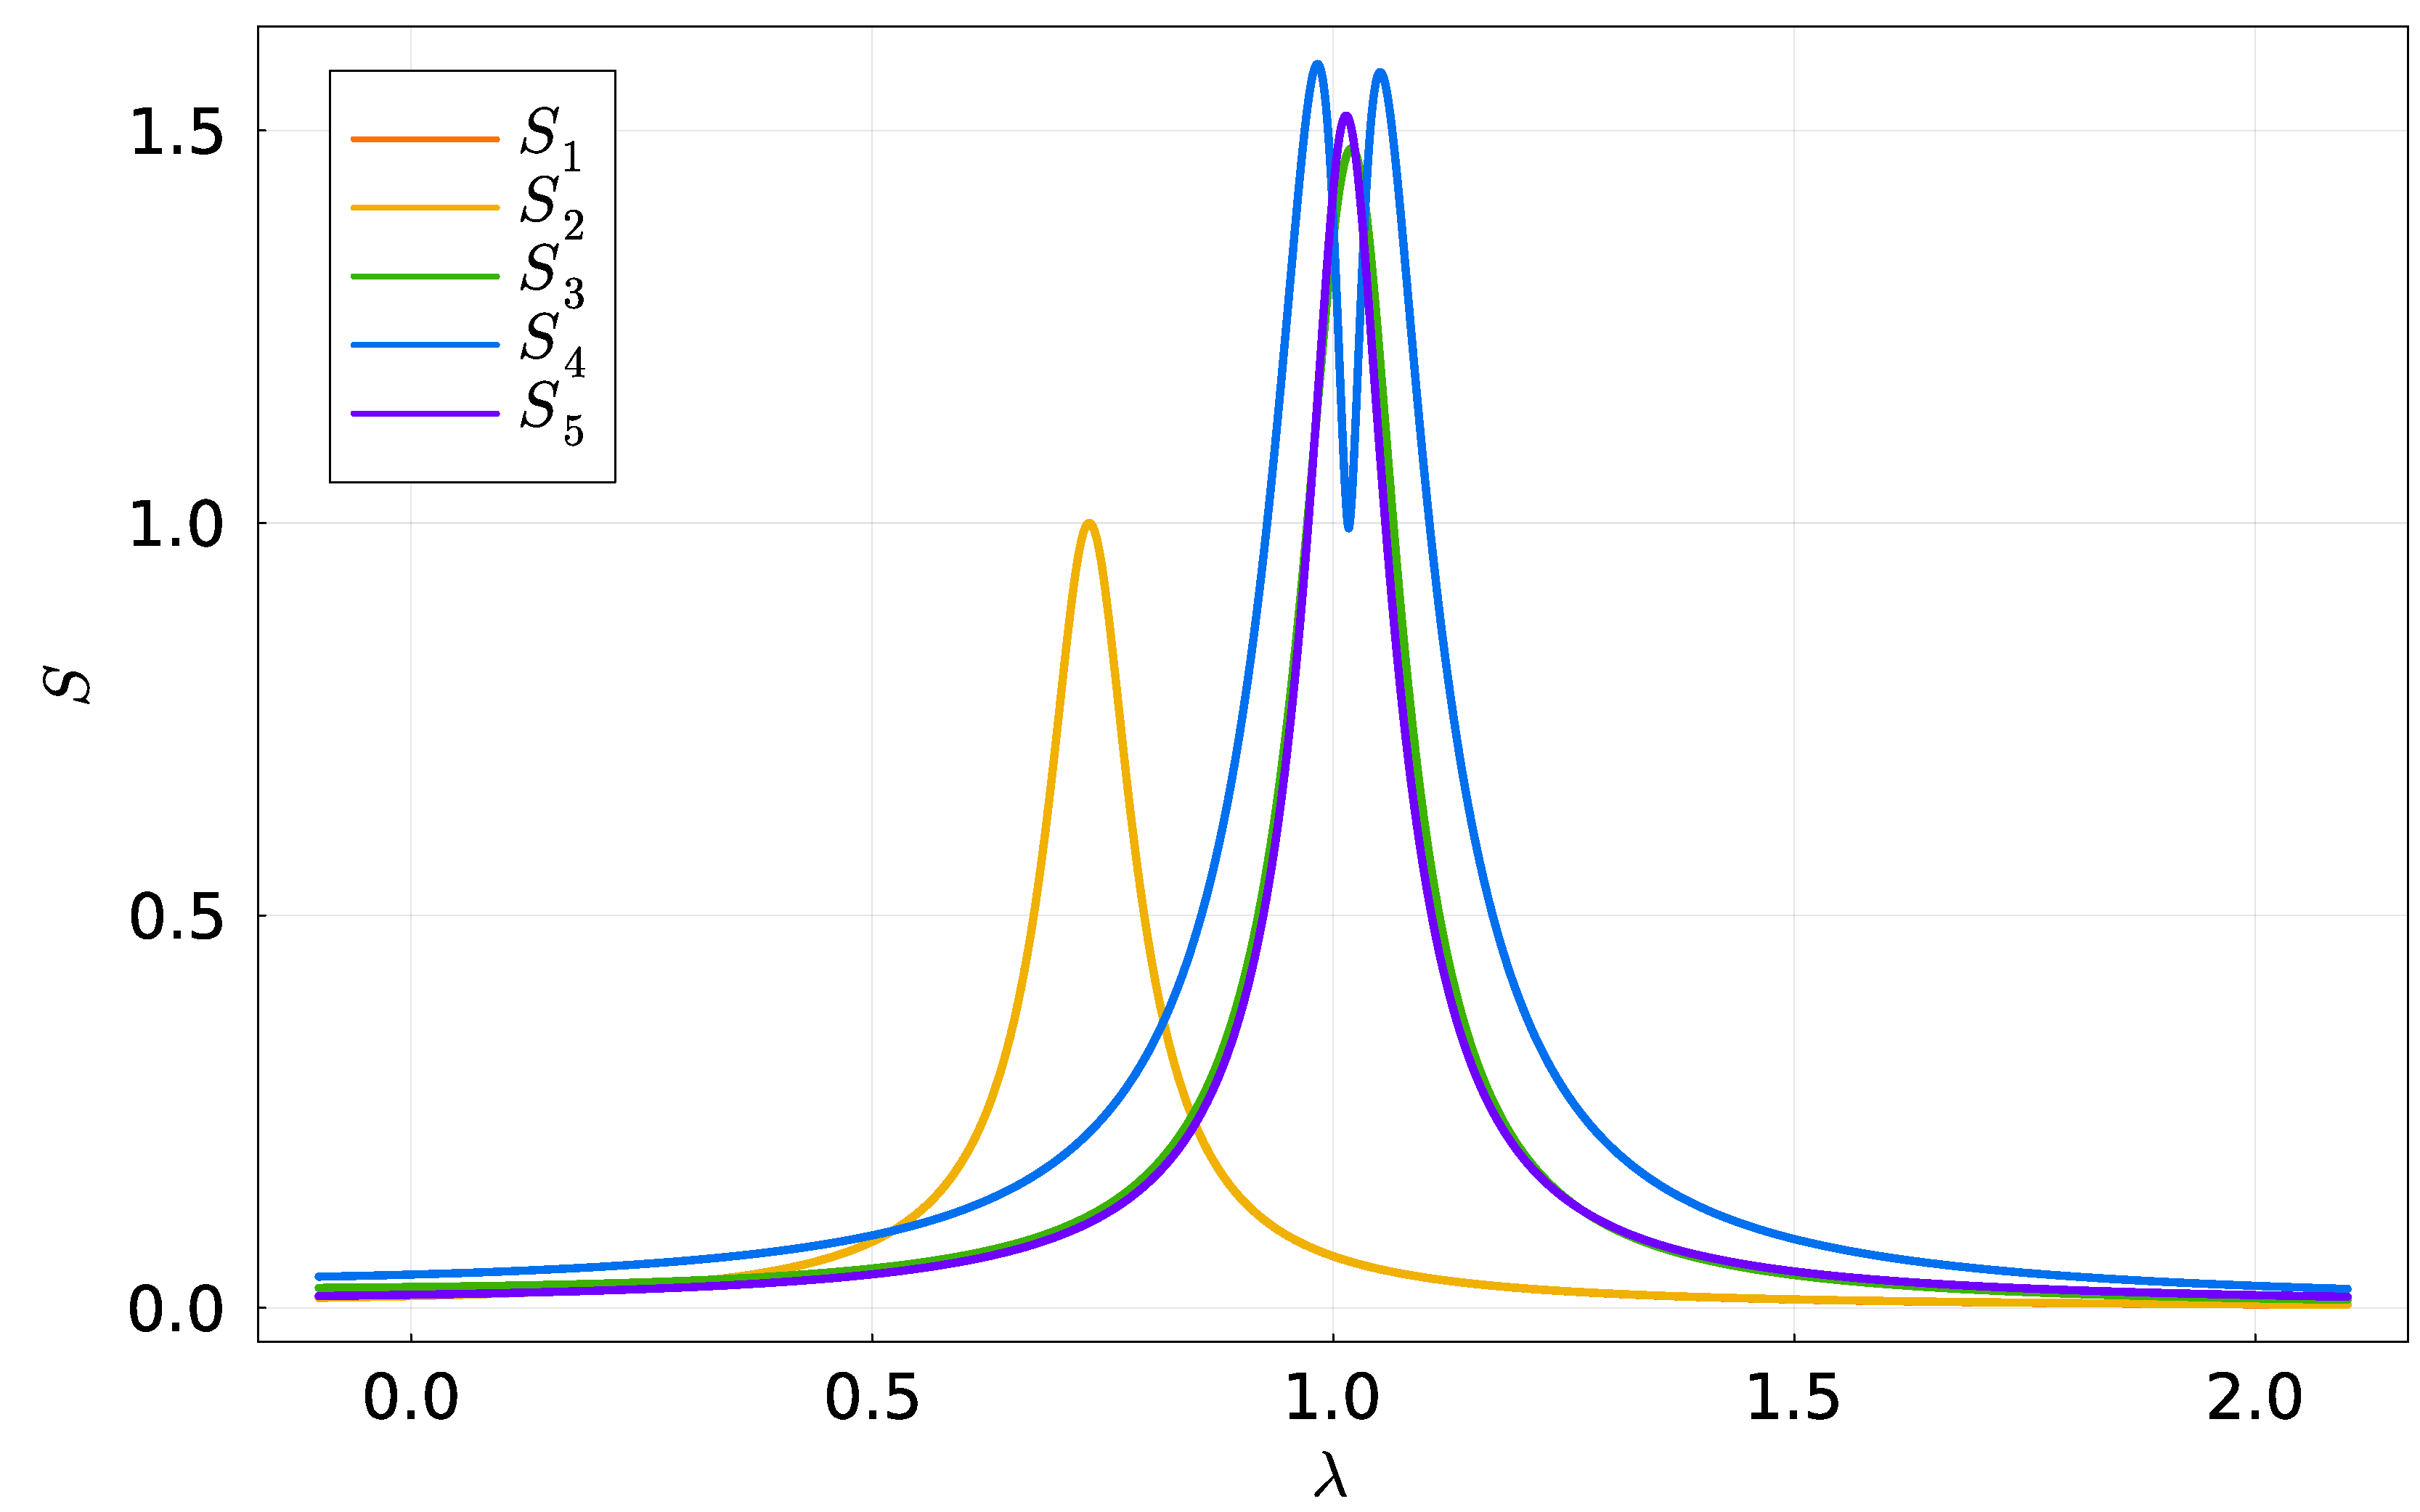
\includegraphics[width=\columnwidth]{figures/figure4.pdf}
        \includestandalone[width=\columnwidth]{figures/figure4}
        \caption{\label{fig:entropies} Numerical results for the von Neumann entropy of the five lowest excited states as a function of the voltage parameter $\lambda$. The entropies $S_1$ and $S_2$ of the $\ket*{\Phi_1}$ respectively $\ket*{\Phi_2}$ states are nearly identical. Note that the peaks in entropy corresponds to the avoided crossings seen in figure~\ref{fig:avoided-crossing}. %But not quite! Why? Or rather why is the triple crossing at lambda slightly larger than 1.
        }
    \end{figure}


    \textbf{Some discussion points:}
    \begin{enumerate}
        \item How can the two avoided crossing points be moved further apart to give
            ``cleaner'' entanglement gates?
        \item Why do we ``only'' use seven anodes? What could be gained by
            increasing this number?
        \item What is the tradeoff in lowering the interaction to get cleaner spikes
            for the entanglement entropy?
        \item What are the limitations of this study?
            Both in terms of the physical limitation of the one-dimensional model,
            and from numerical errors such as the ``kinks'' observed in the wells.
    \end{enumerate}

\section{Conclusions} % we can wait to write this one until the end


\begin{acknowledgments}
We are grateful to M.I. Dykman and S.A. Lyon for illuminating discussions. The work of MHJ is supported by the U.S. Department of Energy, Office of Science, office of Nuclear Physics under grant No. DE-SC0021152 and U.S. National Science Foundation Grants No. PHY-1404159 and PHY-2013047. JP acknowledges support from the National Science Foundation via grant number DMR-2003815 as well as the valuable support of the Cowen Family Endowment at MSU. The work of NRB is supported by a sponsored research grant from EeroQ Corp. JP and NRB thank J.R. Lane and J.M. Kitzman for illuminating discussions. OL has received funding from the European Union's Horizon 2020 research and innovation programme under the Marie Skłodowska-Curie grant agreement Nº 945371.
\end{acknowledgments}


\appendix
\section{Classical two-body calculations}


\bibliography{apssamp}% Produces the bibliography via BibTeX.

\end{document}
%
% ****** End of file apssamp.tex ******
